\chapter{Machine Learning Tools}
\label{ch:ml_tools}

\section{Introduction}
The search for semi-visible jets presents an opportunity to use novel machine learning (ML) tools to uncover patterns in the behavior of dark QCD. The subtlety of the shower differences between dark QCD (signal) and SM QCD (background) motivates a complex model that can accept high-dimensional low-level information, such as particle track information, to understand key differences between signal and background patterns. Additionally, the large number of theory parameters which can be chosen arbitrarily and affect the shape of the dark QCD shower motivate exploring a data-driven machine learning approach, which could be sensitive to a wide variety of dark QCD behavior. \par

To this end, two machine learning approaches are developed for this search, which are used in tandem. The first is a \textit{supervised} ML method where the ML algorithm is built to maximize sensitivity to the specific SVJ signal models described in Section~\ref{subsec:signals}. Here, supervised refers to the use of full and correct \textit{labels}\footnote{In machine learning a label refers to the correct identification information for an input. In the case of the binary classifier algorithm discussed here, the label is either ``signal'' or ``background''.} for all events considered during model training. The second is a semi-supervised method, where training of the model is data-driven (no signal hypothesis used during training) and labels are only partially provided during training. The semi-supervised ML algorithm broadens the discovery sensitivity of the search, and reduces the dependence on the exact theory parameters chosen for signal model simulation. \par

The two different ML algorithms used in this approach will be explored in Section~\ref{subsec:supervised} and Section~\ref{subsec:unsupervised}, along with their application in the SVJ analysis strategy. In the following Section~\ref{sec:ml_fund}, a brief overview of fundamental machine learning concepts is presented.

\subsection{Machine Learning Fundamentals}
\label{sec:ml_fund}

The machine learning tools presented in this chapter depend on two basic \textit{architectures}.
An ML architecture refers to the specific neural network design used to create an ML \textit{algorithm} (or \textit{tool}). 

The first basic architecture is a deep neural network (DNN)~\cite{dnn}.
Figure~\ref{fig:dnn} illustrates the concept.
The hidden layers of a DNN allow the network to store information about the importance of each input feature and the importance of correlations amongst the input features.
The elements of each layer are known as \textit{nodes}.
In a fully connected network like the one shown each node receives input from every node in the previous layer, represented by the arrows in the diagram.
Each node input has an associated \textit{weight} which is adjusted during training.
The node combines the inputs and their associated weights according to an \textit{activation function}.
The output of the activation function becomes the value associated to the node, which is then used as input to the subsequent layer.

\begin{figure}[!htbp]
\centering
   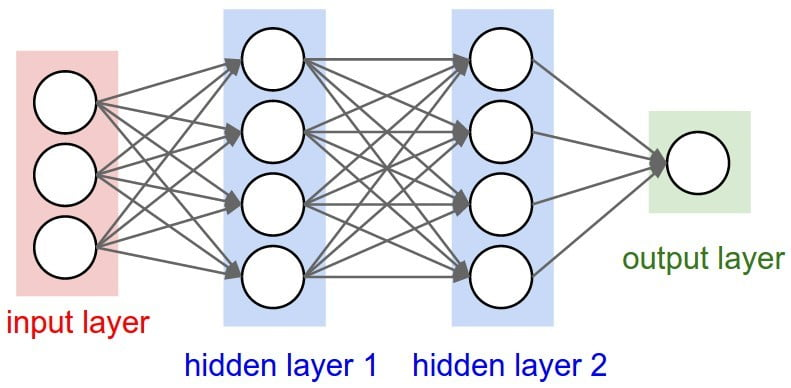
\includegraphics[width=0.7\textwidth]{figures/ml/dnn}
    \caption{A diagram of a deep neural network architecture. 
    \label{fig:dnn}}
\end{figure}

A \textit{loss function} measures the performance of the model. 
The \textit{loss} calculated by the loss function compares the output of the model to the correct response; a lower loss indicates better performance.
In a \textit{classifier} model the output layer is the probability that the input fits a certain category, for example ``signal'' (1.0) or ``background" (0.0).
This probability is called the \textit{score}.
The loss function calculates the accuracy of the scores.
For example a signal input that receives a score of 0.9 would result in a small loss, while the same event given a score of 0.1 would result in a large loss.
Figure~\ref{fig:score_example} illustrates a typical classifier score response.

\begin{figure}[!htbp]
\centering
   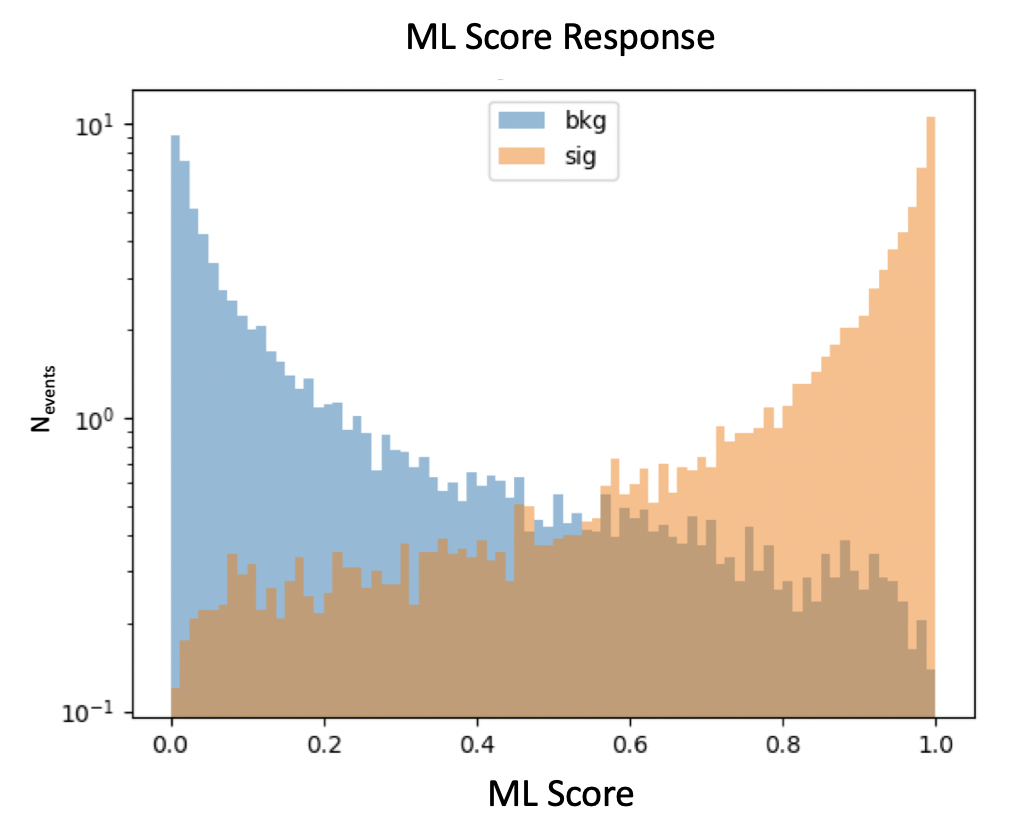
\includegraphics[width=0.5\textwidth]{figures/ml/ml_score_example}
    \caption{An example score distribution for a binary classifier. A higher score indicates a greater probability of the event being signal-like. Most signal events (orange) receive a high score while most background events (blue) receive a low score, indicating good classification.
    \label{fig:score_example}}
\end{figure}

The network improves by training over many \textit{epochs}, which refers to the process of the ML algorithm evaluating all training events.
After each epoch, the \textit{optimizer} adjusts the weights to reduce the loss.
The \textit{learning rate} determines how big of an adjustment the network is allowed to make. 
During training, a set of events are set aside to use for \textit{validation}.
The purpose of the validation data is to prevent \textit{overtraining}.
If a network is sufficiently large and complex, the network could lose generality by perfectly learning (or ``memorizing'') the correct response for every training event.
This would minimize the training loss, but could result in the network failing to correctly classify events it hasn't seen before. 
By evaluating the loss of the validation data the user can determine if the network is overtrained; the validation loss should not greatly exceed the training loss.

ML algorithms are often evaluated through a \textit{receiver operating characteristic} (ROC). 
The ROC compares the true positive rate (correct classification) with the false positive rate (false classification).
An example ROC curve is shown in Figure~\ref{fig:roc}. 
If a classifier is performant, the true positive rate will be larger than the false positive rate for all possible false positive rates.
If the network has no classifying power, the true positive rate and false positive rate will be equal throughout.
The \textit{area under the curve} (AUC) is an important metric for evaluating the ROC.
The AUC is the integral of the ROC curve.
An AUC of 1.0 indicates perfect performance, while an AUC of 0.5 indicates that the network is no better than random guessing.

\begin{figure}[!htbp]
\centering
   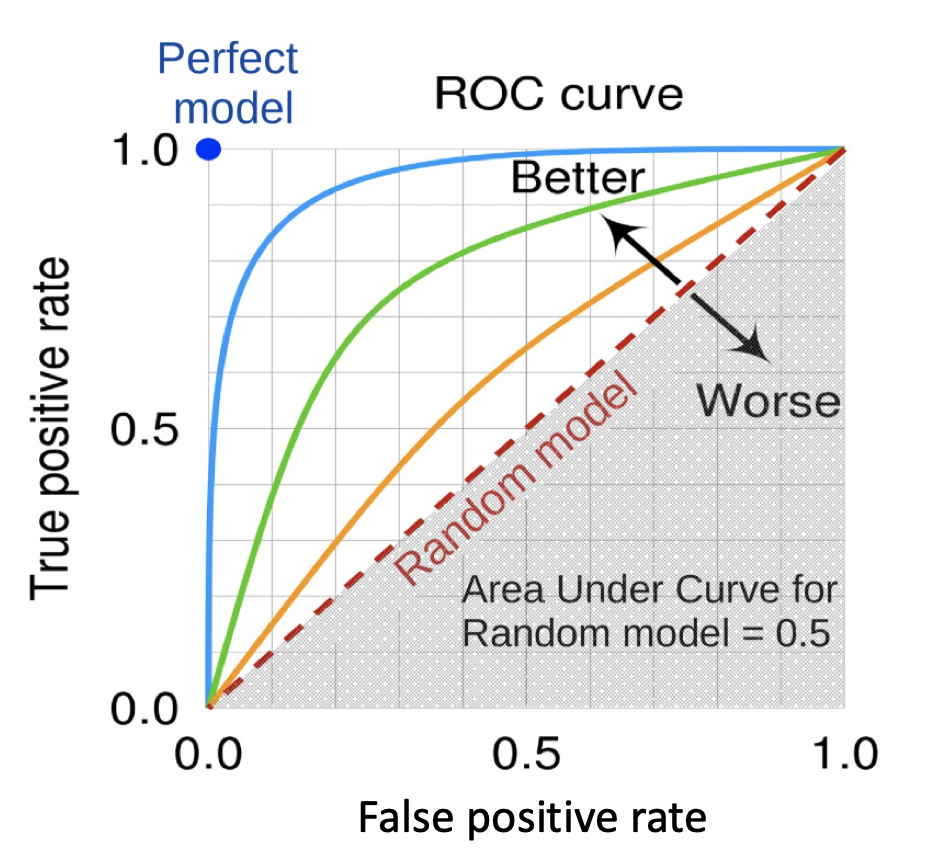
\includegraphics[width=0.6\textwidth]{figures/ml/roc_example}
    \caption{Several example ROC curves. The AUC is also illustrated \cite{auc_example}.
    \label{fig:roc}}
\end{figure}

The second architecture that is important to this thesis is the auto-encoder (AE)~\cite{autoencoders}. 
Unlike a DNN, which is a supervised network that depends on the use of correct labels to determine the loss, the AE calculates loss by comparing the input and output layers.
Figure~\ref{fig:ae} illustrates the concept.
The network is designed to extract the most salient features of the input via dimensionality reduction.
This is achieved by compressing the input to a lower dimensional \textit{latent space}, and then attempting to reconstruct the original input from that latent space.
The loss is calculated by comparing the output of the network with the input.
While the goal of a classifier is to correctly categorize the inputs, the goal of the AE is to correctly reconstruct the inputs.
This allows the AE to be used for \textit{anomaly detection}.
The kinds of events that are seen most often during training will be reconstructed well by the algorithm, and therefore have the smallest loss.
Events which are anomalous or unusual in the training data will be more difficult for the AE to reconstruct, and therefore receive a larger loss. 
The loss can be used to create an \textit{anomaly score}, which identifies unusual events with a higher anomaly score.

\begin{figure}[!htbp]
\centering
   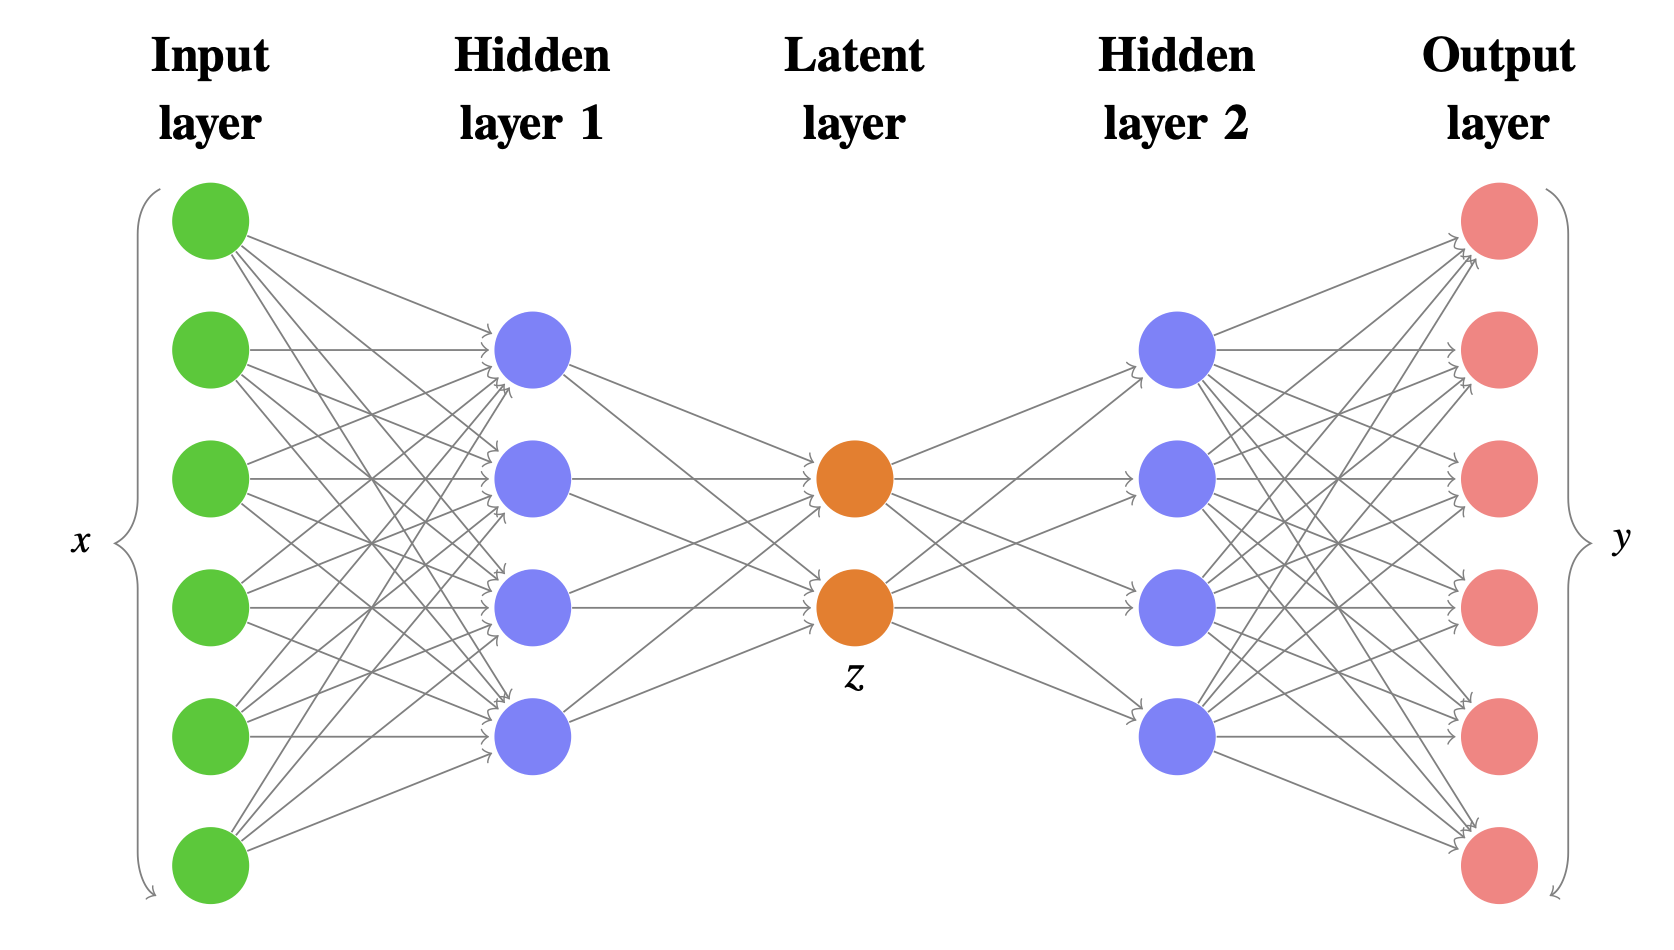
\includegraphics[width=0.7\textwidth]{figures/ml/ae}
    \caption{A diagram of auto-encoder architecture. The loss is computed as a difference (often the \textit{mean squared error} or MSE) between the input x and the output y \cite{vrnn}.
    \label{fig:ae}}
\end{figure}



%------------------------------------------------
\section{Particle Flow Network (Supervised)}
\label{subsec:supervised}
The supervised machine learning approach maximizes discovery sensitivity for the SVJ signals considered in this thesis.
The networks learns the features of the SVJ signals, allowing the network to be highly efficient in selecting events that resemble the SVJ signal.

\subsection{Architecture Fundamentals}

A Particle Flow Network (PFN)~\cite{pfn} architecture is selected for two reasons: \textit{permutation invariant input modeling} to best describe the events consisting of an unordered set of particles, and a \textit{low-level input modeling} to take advantage of the ability of neural networks to uncover patterns in high-dimensional data. \textit{Low-level} refers to using detector level information such as individual particle tracks, rather than \textit{high-level} information such as reconstructed jet objects. Low-level inputs are generally high-dimensional; for instance, an event may have only 2 jets (dim-2), but each jet consists of 70 particles (dim-140). Low-level input modeling is chosen to capture the intricacies of dark QCD showers with may not express themselves in high level objects, as explored in Ref.~\cite{darkqcd}. Permutation invariant input modeling is chosen as the most accurate representation of a set of particles. In previous work such as Ref.~\cite{vrnn}, ordered input modeling has been observed to \textit{bias} the performance of low-level modeling tools. In this case bias means that the performance of the tool was observed to change substantially depending on the input ordering; however, there is no physics motivation for choosing any particular order. 

The input to the PFN is a collection of particles and their associated physics information, such as momentum and trajectory. Constructing the PFN involves the creation of new basis variables $\Phi$ for each particle in the input event. This transformation is summarized as $\vec{p_i} \rightarrow \vec{\Phi_i}$ where $\vec{p_i}$ is the physics information for the $i$th particle in the event, and $\vec{\Phi_i}$ is that same information encoded into the $\Phi$ basis. Permutation invariance is enforced by summing over the $\Phi$ basis for every particle in the event to create a new permutation invariant event representation $\mathcal{O}$. The creation of $\mathcal{O}$ from $M$ particles $\vec{p}$ with $d$ physics features each can be expressed as:

\begin{equation}
  \mathcal{O}(\{\vec{p_1},...,\vec{p_M}\}) = \sum_{i=1}^M \Phi_i(\vec{p_i})
  \label{eq:pfn}
\end{equation}

where $\Phi : \mathbb{R}^d \rightarrow \mathbb{R}^l$ is a per particle mapping, with $l$ being the dimension of the new basis $\mathcal{O}$. Figure~\ref{fig:pfn_paper} gives a graphical representation of the use of summation in the PFN over per-particle information to create a permutation-invariant event representation. \par
\begin{figure}[!htbp]
\centering
   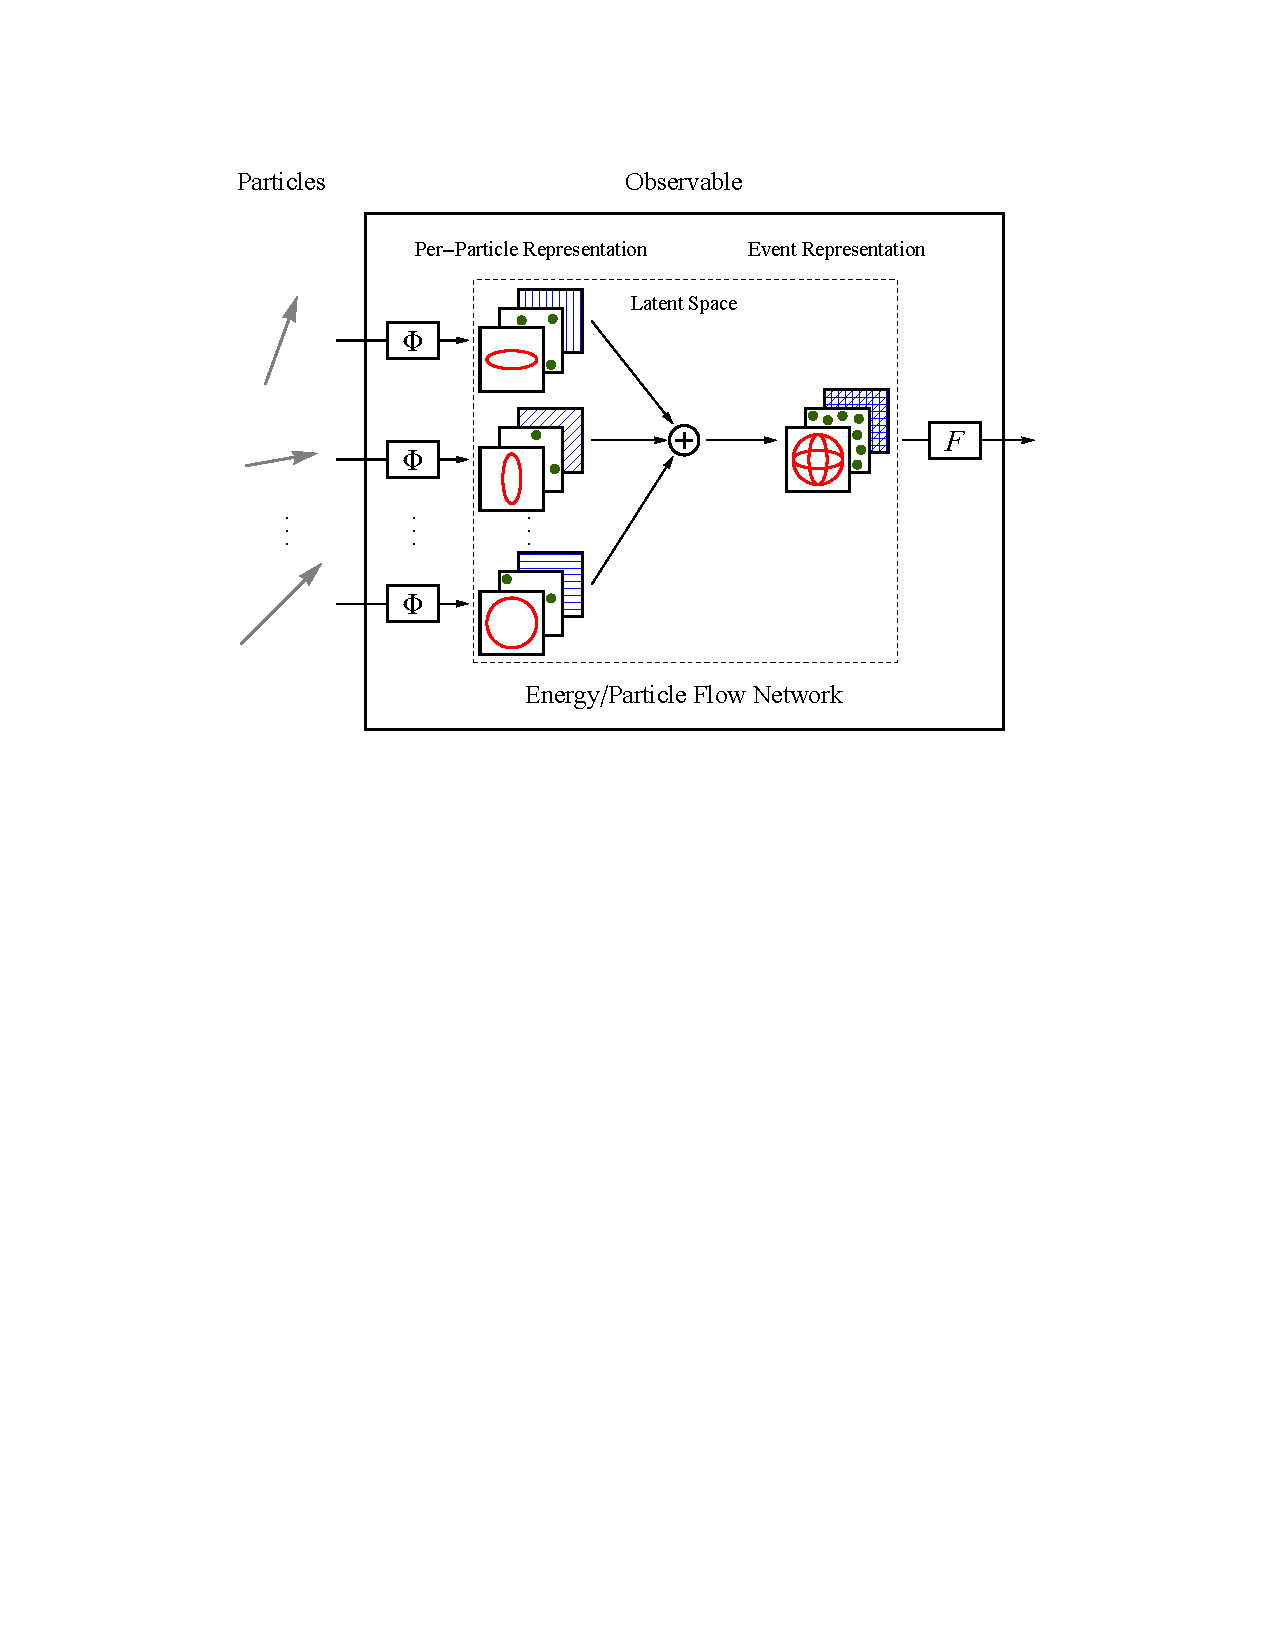
\includegraphics[width=0.7\textwidth]{figures/ml/pfn_paper}
    \caption{The Energy/Particle Flow Network concept, from Ref.~\cite{pfn}. The physics input information is represented as arrows on the left, for an arbitrary number of particles. The $\Phi$ transformation converts these arrows to 3 graphs, indicating the $\Phi$ basis dimension $l$ is 3 in this example. The graphs are then summed for all particles to create $\mathcal{O}$, or the event representation.
    \label{fig:pfn_paper}}
\end{figure}

The $\Phi$ basis transformation is implemented via a deep neural network. The output of the neural network is summed as indicated in Equation~\ref{eq:pfn} to create the new permutation invariant event representation $\mathcal{O}$. $\mathcal{O}$ then becomes the input of a second deep neural network $F$. $F$ is a classifier network which separates signal and background events. Figure~\ref{fig:pfn_arch} provides an annotated diagram of the PFN architecture as used in this analysis. 
\begin{figure}[!htbp]
\centering
   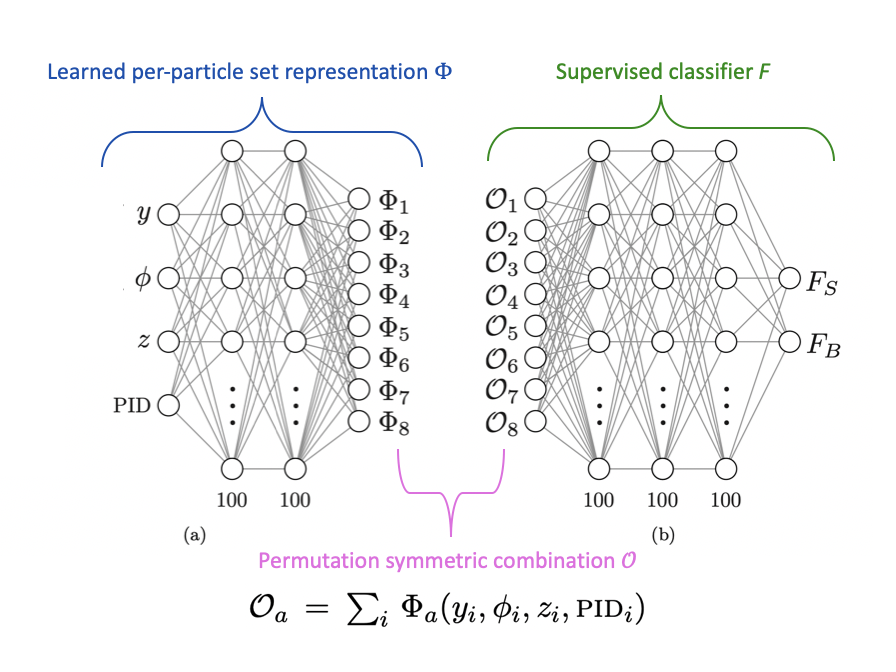
\includegraphics[width=0.8\textwidth]{figures/ml/pfn_arch}
    \caption{An annotated diagram of the PFN architecture~\cite{pfn}. $y$ and $\phi$ represent geometric trajectory information for the input particles, $z$ represents energy information, and PID encompasses any other particle ID information in the input. PID is presented in the diagram as a 1-dimensional input, but could represent multiple input dimensions.
        \label{fig:pfn_arch}}
\end{figure}

%--------------------
\subsection{Input Modeling, Scaling, and Rotation}
\label{sec:input_model}
In this implementation, the particle input information comes from all tracks associated to the leading and subleading jets. The track association method is Ghost association, as discussed in Section~\ref{sec:ghost}. A single jet tagger strategy was also considered, but utilizing tracks from both leading jets creates a more complete low-level picture of the event. The choice of the two leading jets is justified in Chapter~\ref{ch:analysis}. If we consider the dijet topology of semi-visible jets as illustrated in Figure~\ref{fig:svj_pic}, the advantage of modeling both leading jets simultaneously becomes clear. In the semi-visible jet model presented in Ref.~\cite{darkqcd}, \met~in the event is expected to arise due to an imbalance in the number of visible tracks of the two jets associated to the dark quark decay.\par

\begin{figure}[!htbp]
\centering
   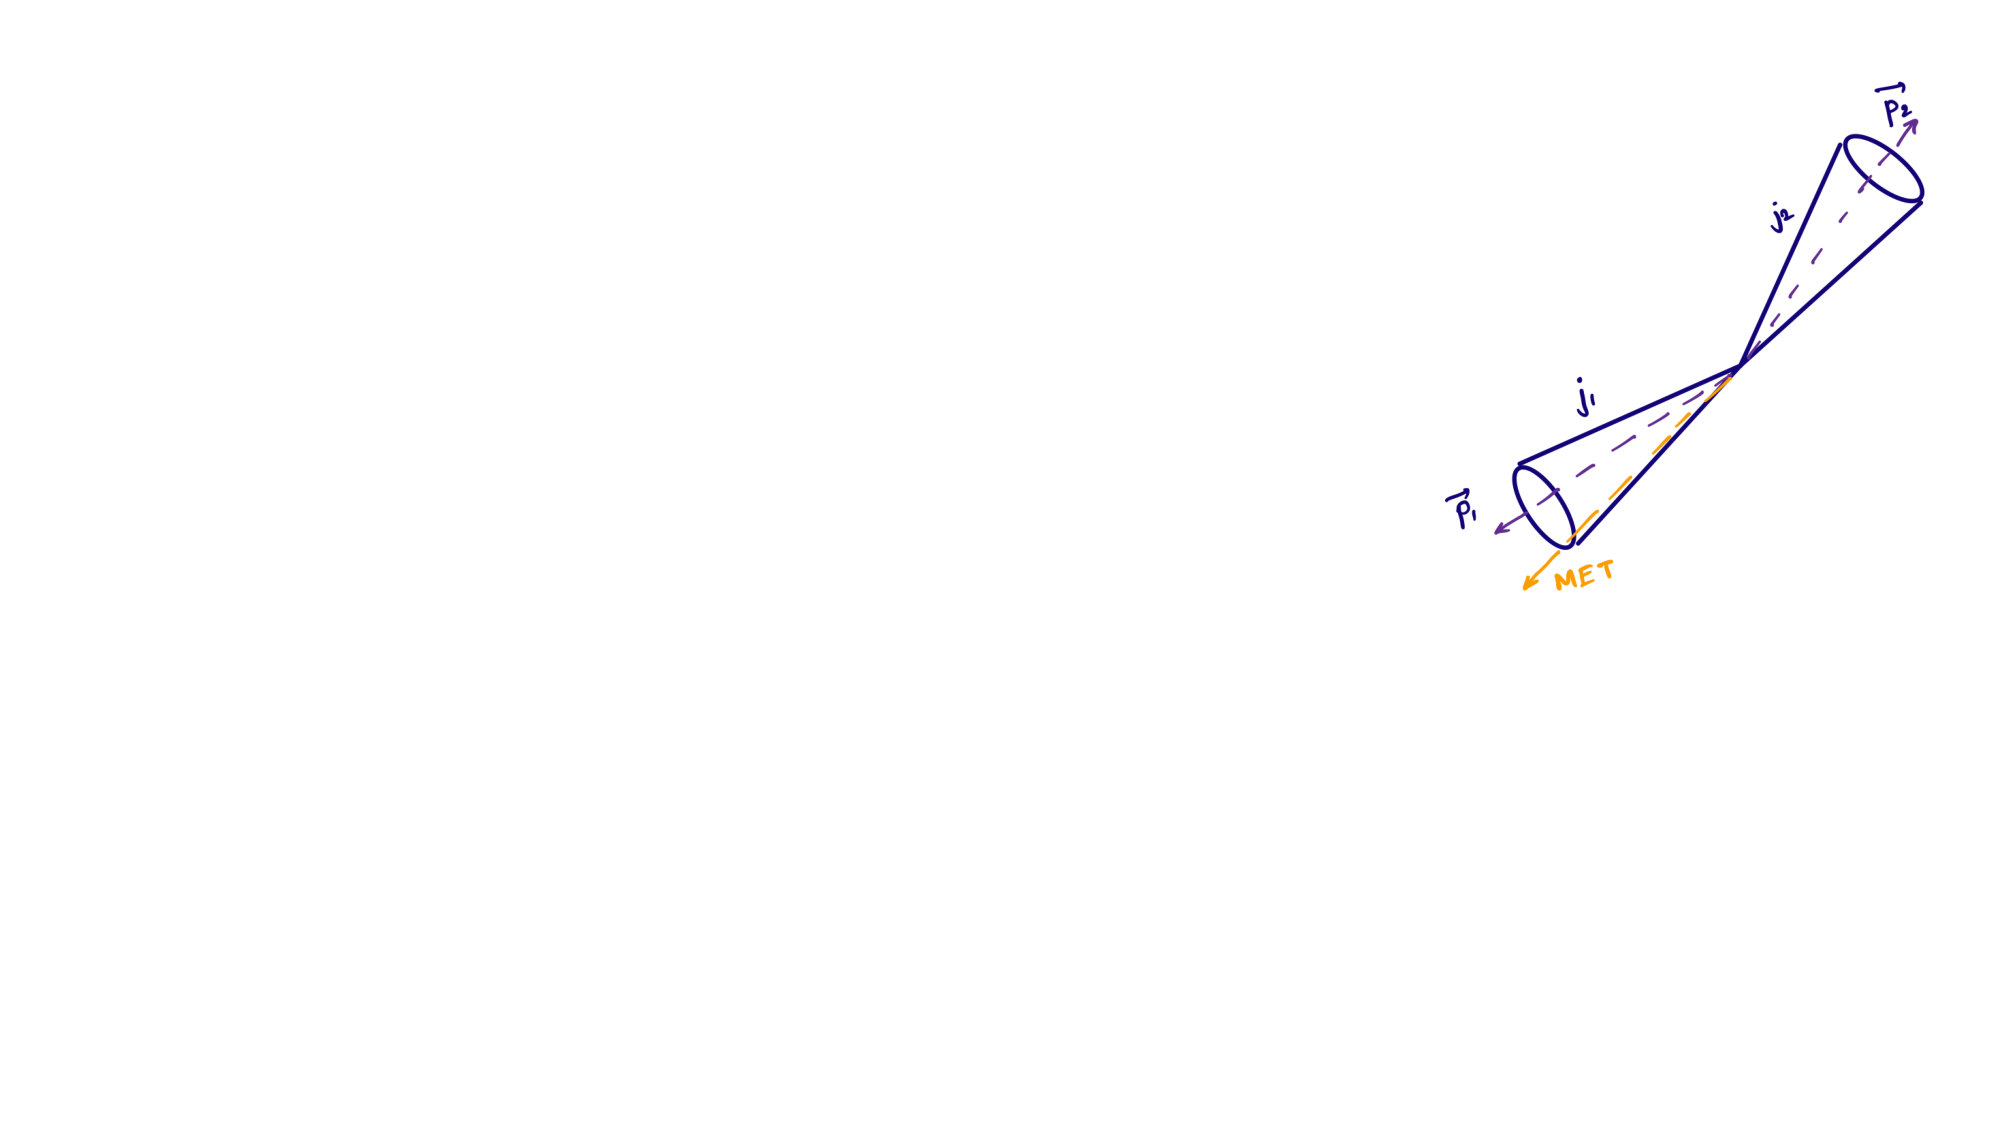
\includegraphics[width=0.4\textwidth]{figures/ml/dijet_topology}
    \caption{An illustration of the expected dijet behavior of semi-visible jets, where one jet is closely aligned with \met (MET). In the figure two jet cones $j_1$ and $j_2$ are illustrated, along with their associated momentum vectors $\vec{p_1}$ and $\vec{p_2}$. 
        \label{fig:svj_pic}}
\end{figure}

Each track is described using six variables: the four-vector of the track (\pt, $\eta$, $\phi$, E), and the track displacement parameters $d_0$ and $z_0$, where $d_0$ measures displacement in the radial direction from the beamline and $z_0$ measures displacement along the beamline from the primary interaction point. Figure~\ref{fig:trackcoordinates} illustrates these coordinates. Up to 80 tracks per jet are allowed, which is a threshold chosen to generally include all the tracks in the jet, which leads to maximal performance.\par %Figure~\ref{fig:ntracks} shows the track multiplicity in the leading and subleading jet for the signal and background samples used in training. \par

\begin{figure}[!htbp]
\centering
   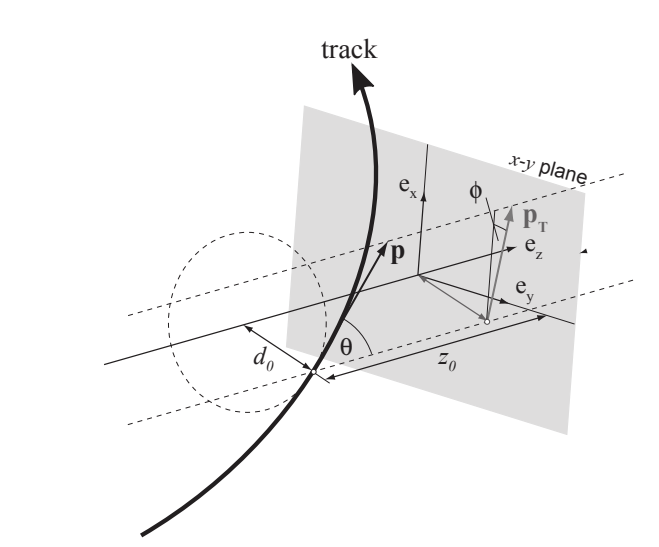
\includegraphics[width=0.4\textwidth]{figures/ml/trackcoordinates}
    \caption{Illustration of track coordinates $d_0$ and $z_0$.
    \label{fig:trackcoordinates}}
\end{figure}

%\begin{figure}[!htbp]
%\centering
 %  \includegraphics[width=0.95\textwidth]{figures/ml/ntracks}
 %   \caption{Distributions of the track multiplicity in the leading and subleading jets, comparing signal and background PFN training samples.
%    \label{fig:ntracks}}
%\end{figure}

These tracks (up to 160 total) are the input to the PFN. Referencing Equation~\ref{eq:pfn}, this corresponds to $M = 160$ (number of particles) and $d = 6$ (number of features per particle). The two leading jets and their associated tracks are rotated so that the vector sum of the jets, or system average, is aligned with $(\eta,\phi) = (0,0)$. The rotation can be summarized as 
\begin{subequations}
    \begin{align}
       \eta_{i}' &= \eta_i - \bar{\eta},  \\
        \phi_{i}' &= \phi_i - \bar{\phi}
    \end{align}
\end{subequations}
where ($\bar{\eta}, \bar{\phi}$) is the average angle of the dijet system,  ($\eta_{i}, \phi_{i}$) are the original track coordinates, and ($\eta_{i}', \phi_{i}'$) are the rotated track coordinates. Figure~\ref{fig:jet_rotate} illustrates the rotation process. The rotation ensures that the information used by the algorithm is the relative orientation of the jets (and associated tracks) to each other, not their absolute position in the detector. Each track is normalized to its relative fraction of the total dijet system energy and transverse momentum; this enforces agnosticism to the total energy and transverse momentum of the event. The rotation and scaling are motivated by the procedures described in Ref.~\cite{pfn} to improve the performance of the PFN. 

\begin{figure}[!htbp]
\centering
   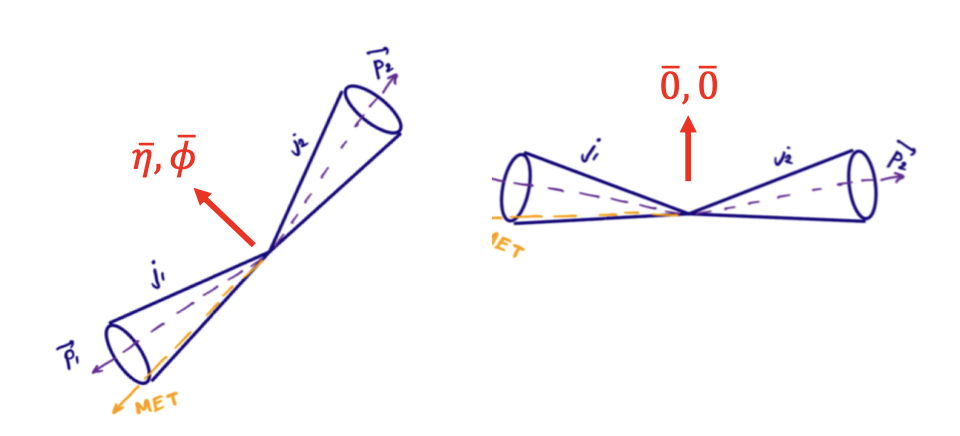
\includegraphics[width=0.65\textwidth]{figures/ml/jet_rotate}
    \caption{A diagram demonstrating how the two jet system is rotated in $(\eta,\phi)$. The jet cones and associated jet tracks are illustrated. The dashed tracks represent dark hadrons while the solid tracks represent SM hadrons. The system average $(\bar{\eta},\bar{\phi})$ is shown in red and an example track with coordinates $(\eta_i,\phi_i)$ is shown in purple.
    \label{fig:jet_rotate}}
\end{figure}

Finally, each of the 6 track variables is scaled so that its range is [0,1]. This is a common preprocessing step that ensures the input data is bounded over a similar range, so that arbitrarily large values don't develop an outsized impact on the model. The track momentum and energy normalization mentioned above naturally enforces that these values are restrained between [0,1]. The $\eta$ and $\phi$ values are naturally bounded, so for these values the $\eta$ tracking range\footnote{This range is dictated by the $|\eta|$coverage range of the Inner Detector, as shown in Table~\ref{tab:atlas_requirements}} of [-2.5, 2,5] and the full $\phi$ range [$-\pi$, $\pi$] are mapped to [0,1]. The displacement variables are restricted to [0,1] via the standard \textsc{MinMaxScaler}~\cite{scikit-learn} method which determines the minimum and maximum values observed in training, and maps those boundaries to 0 and 1 respectively. \par

Figure~\ref{fig:pfn_datamc_input} illustrates that the data is well modeled by the MC at track level. Figure~\ref{fig:pfn_bkgsig_input_kin} shows the kinematics of each of 6 track variables for background and signal. Figure~\ref{fig:pfn_bkgsig_input_rot} shows each of the 6 track variables after scaling and rotation have been applied, demonstrating the impact of these procedures, as well as the track level similarities and differences between the background SM QCD processes and the signal SVJ processes. \par

The $\phi$ distribution is of note for its jagged appearance in QCD MC. This arises due to dead tile calorimeter cells in certain $\phi$ regions, the effects of which are seen in data and modeled in QCD MC but not modeled in SVJ signal MC. Appendix~\ref{subsec:tileCal} contains more information about how the issue was addressed in data. The distribution is not of concern for the PFN training because of the rotation process, which replaces the information about absolute detector $\phi$ measurements with the relative $\phi'$ measurement. This is illustrated in Figure~\ref{fig:pfn_bkgsig_input_rot}, where it is observed that for both signal and background the tracks are clustered back to back, centered at $-\pi$/2 and $\pi$/2 (0.25 and 0.75 after scaling). The only remaining difference is that the signal tracks are more likely to be close to the system average $\bar{\phi}$ than the background jet tracks. This is demonstrated by the excess of signal events in the center of the $\phi'$ plot. This orientation difference is a real feature of the signal model, confirmed in Figure~\ref{fig:presel_vars2} which illustrates that signal jets are more likely to have low $\Delta\phi$ than background jets. 

\begin{figure}[!htbp]
   \centering
   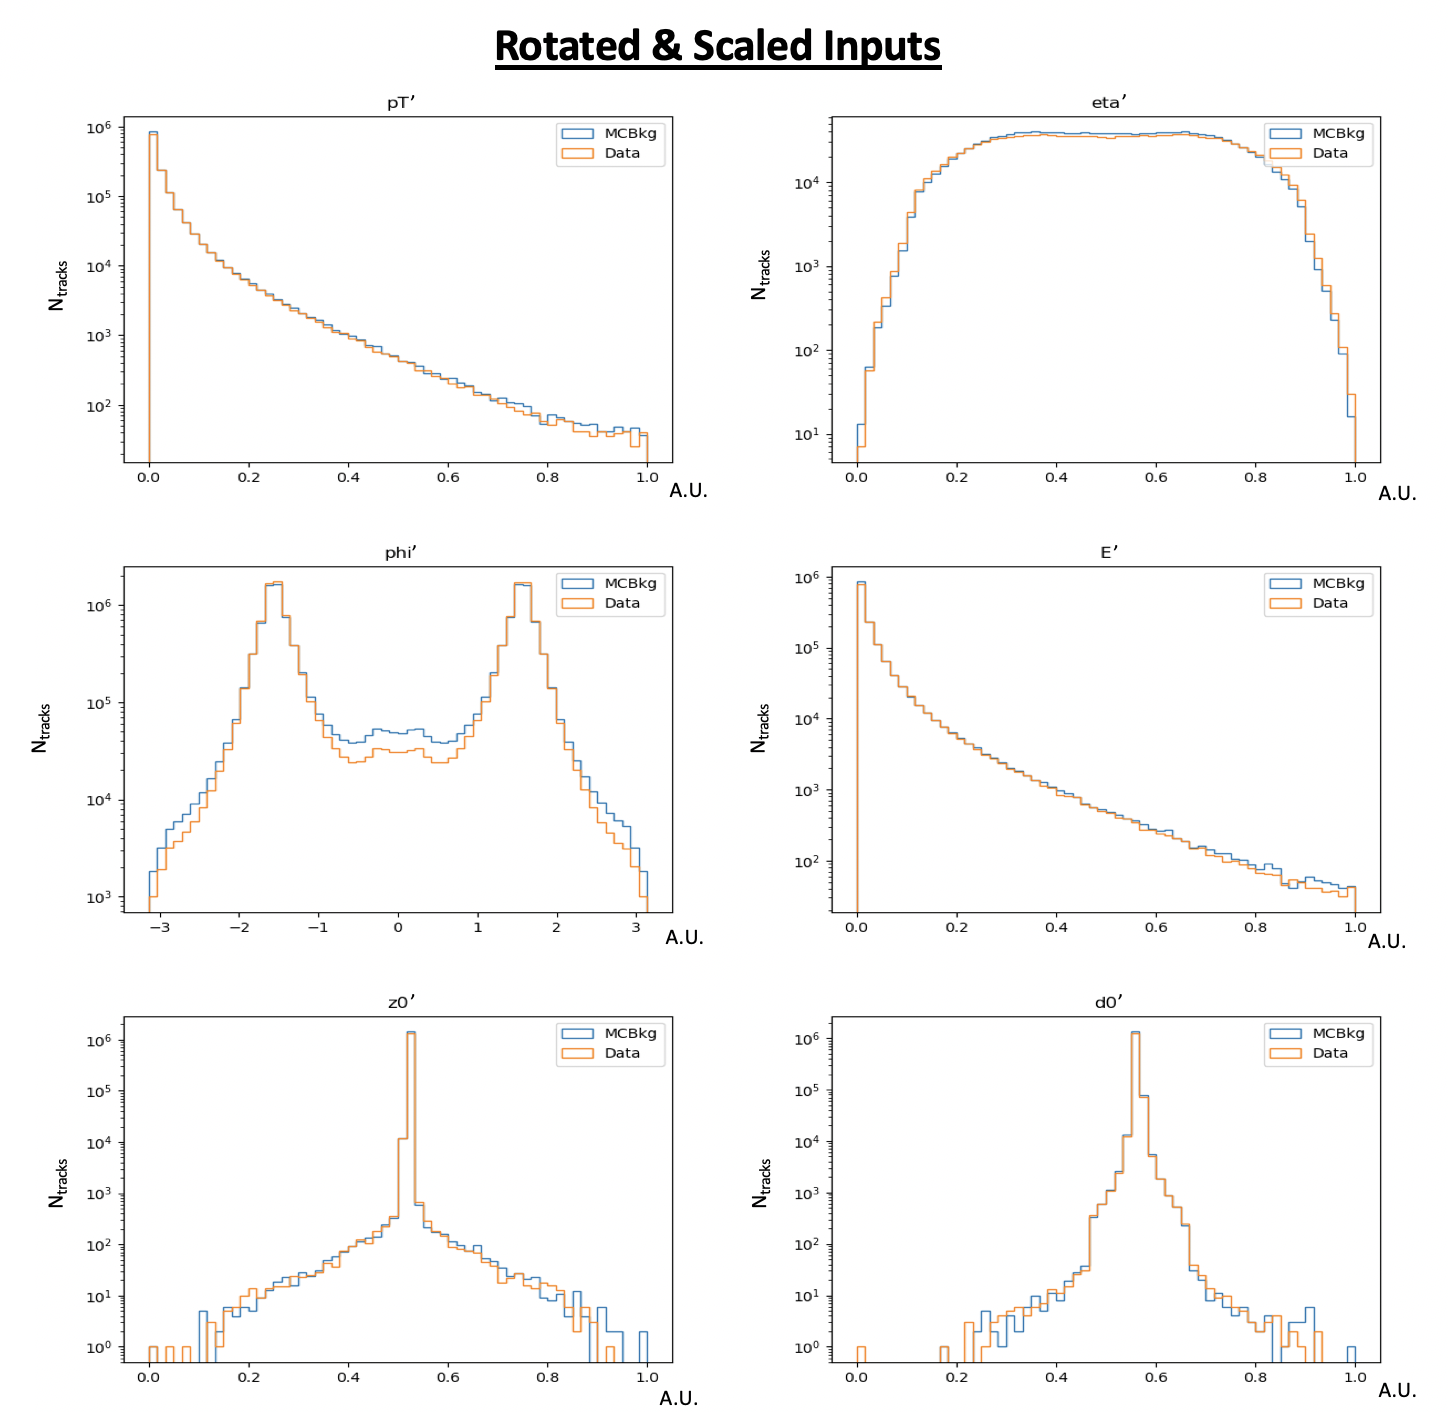
\includegraphics[width=0.99\textwidth]{figures/ml/pfn_datamc_input}
    \caption{The 6 PFN track variables in background MC (blue) and data (orange), after the scaling and rotation procedure is applied. There is excellent modeling of the data by the MC within the track variables. The slight discrepancy in the $\phi$ distribution due to the inaccuracies of modeling dead TileCal cells in the QCD MC is considered. The level of discrepancy is determined to be within tolerance given that the final result with be data driven and the QCD model is used in the PFN training only.
    \label{fig:pfn_datamc_input}}
\end{figure}

\begin{figure}[!htbp]
    \centering
     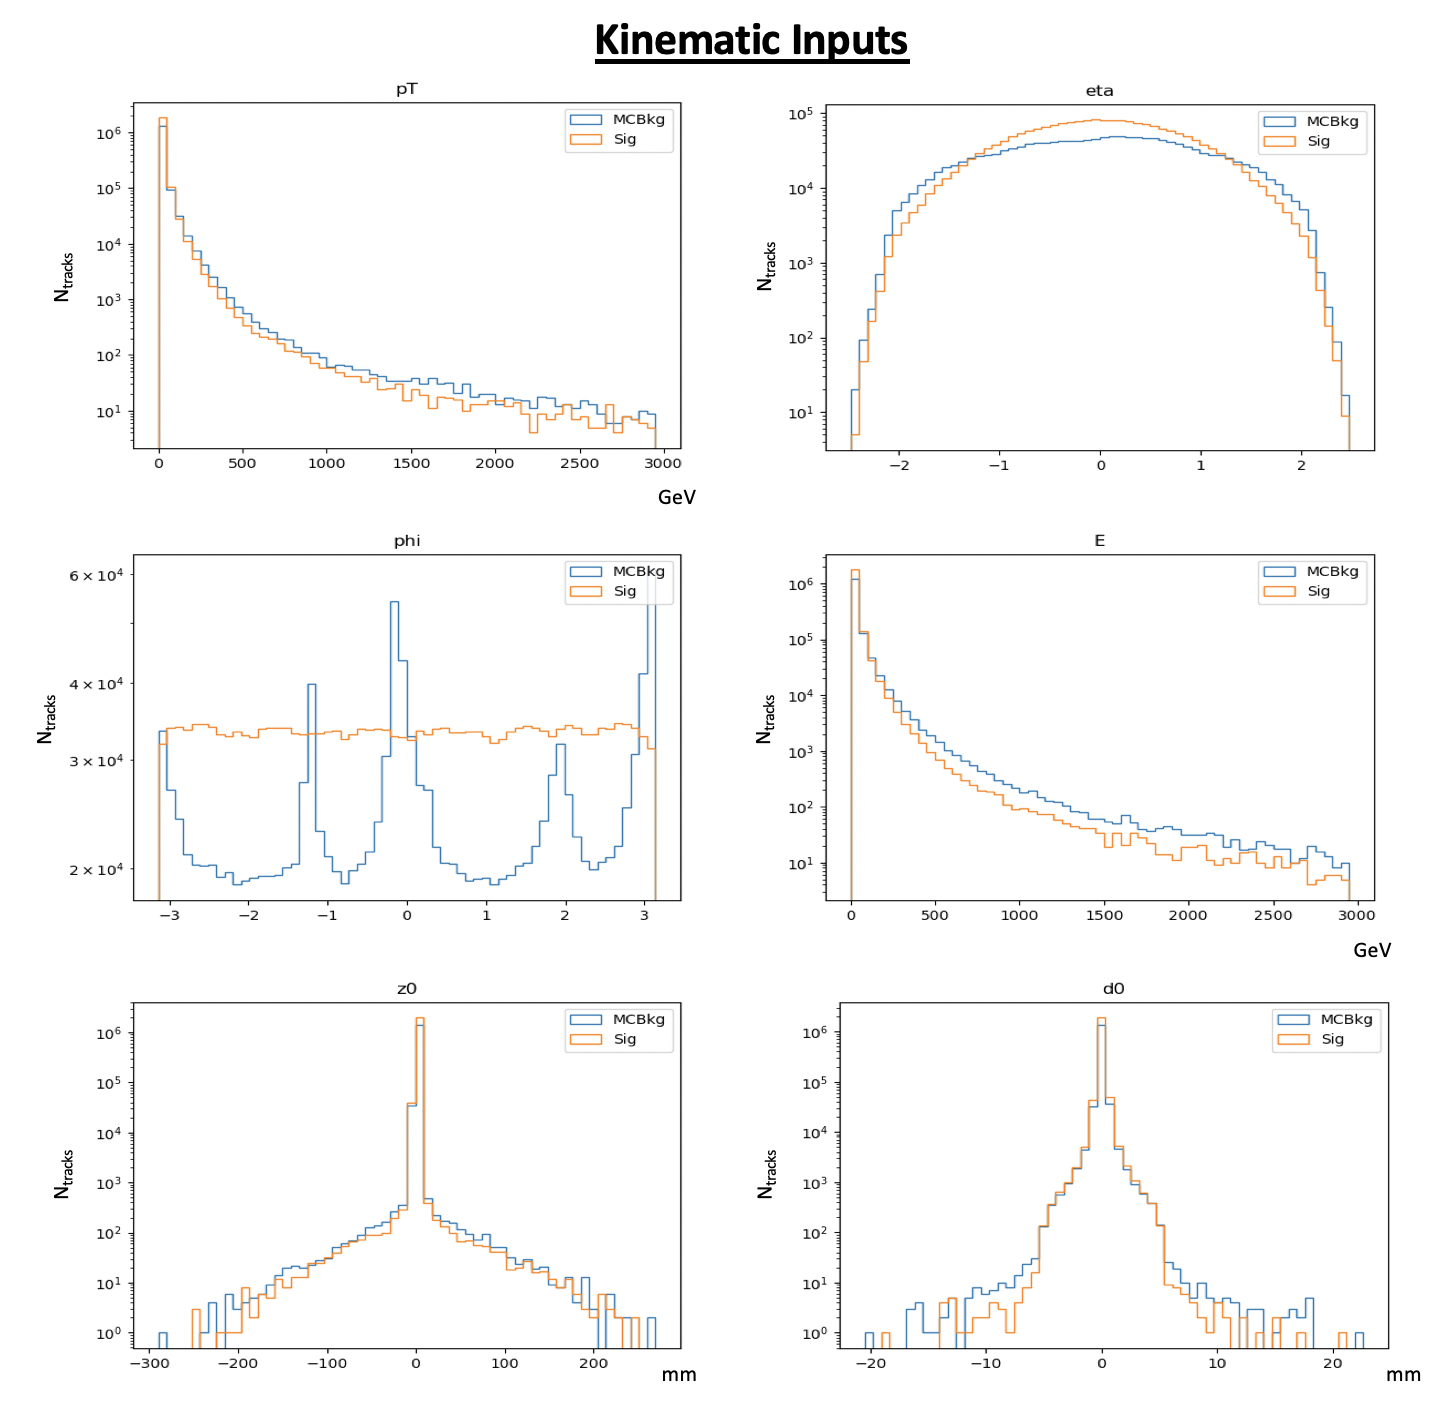
\includegraphics[width=0.99\textwidth]{figures/ml/pfn_bkgsig_input_kin}
     \caption{The 6 PFN track variables in background MC (blue) and signal MC (orange) before scaling and rotation. The track kinematics are largely similar, and the variation in the $\phi$ distribution is explained in the text.}
      \label{fig:pfn_bkgsig_input_kin}
\end{figure}

\begin{figure}[!htbp]
    \centering
    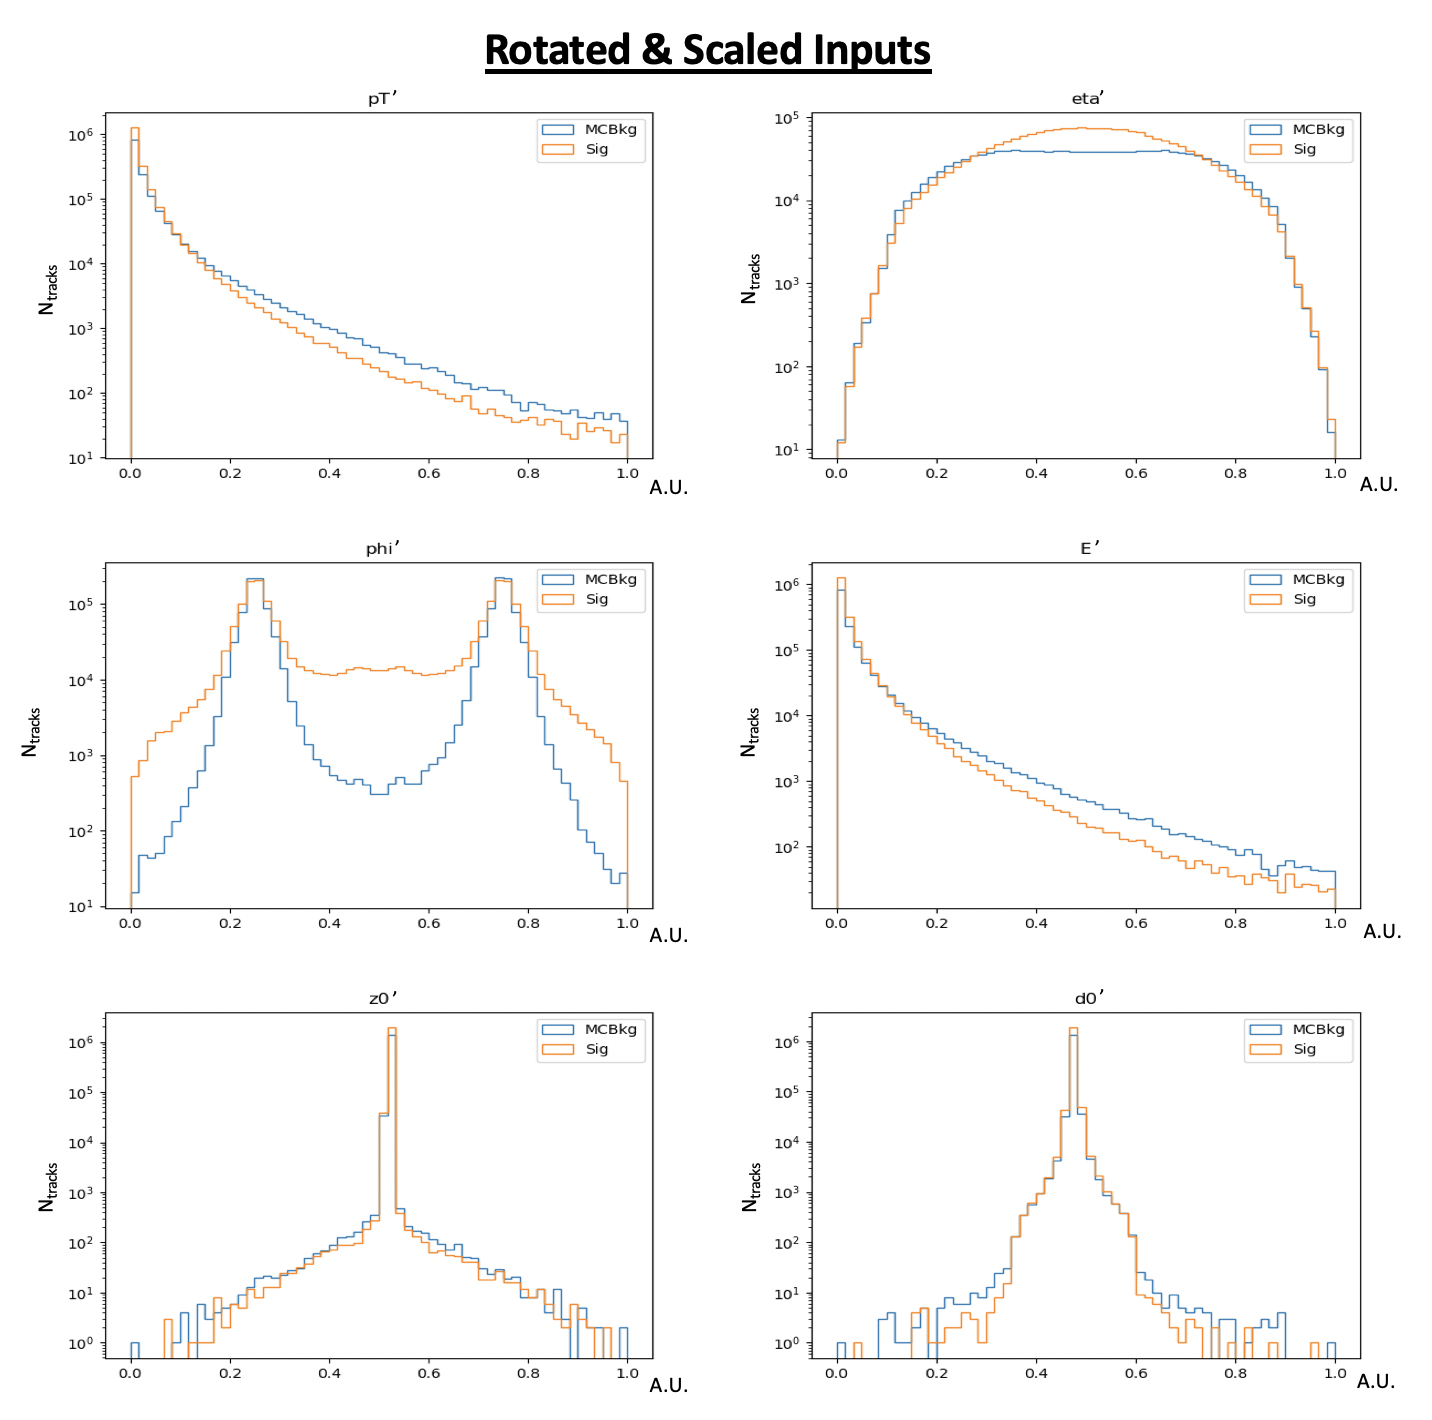
\includegraphics[width=0.99\textwidth]{figures/ml/pfn_bkgsig_input_rot}
     \caption{The 6 PFN track variables in background MC (blue) and signal MC (orange) after scaling and rotation. The $\phi$ distribution is modified by the rotation procedure, as explained in the text.}
     \label{fig:pfn_bkgsig_input_rot}
\end{figure}

\clearpage

%--------------------
\subsection{Training}
\label{sec:pfn_training}

As seen in Figure~\ref{fig:pfn_arch}, two networks are defined and combined for the PFN architecture. In our implementation the input layer has a dimension of 6, accounting for the 6 track variables described in the previous section. The first network, termed the $\Phi$ network, creates the per-particle set representation as illustrated in Figure~\ref{fig:pfn_paper}. The $\Phi$ network has 2 hidden layers each of dimension 75, and an output later of dimension 64. These dimensions were chosen via an optimization procedure which balanced network complexity (achieved with more dimensions) against training time (achieved with fewer dimensions). The two hidden layers and $\Phi$ output layer all use a \textsc{relu} activation function~\cite{scikit-learn}, following the work of Ref.~\cite{pfn}. 

The input layer of the classifier $F$ network is required to have the same dimension as the output layer of the $\Phi$ network, and therefore takes dimension 64. This network contains 3 hidden layers with 75 nodes each, and again uses \textsc{relu} activation~\cite{scikit-learn}. The final layer is the binary classifier result with dimension 2, which uses a \textsc{softmax} activation~\cite{scikit-learn} that is well suited for classification. The loss function for the complete PFN network is \textsc{CategoricalCrossentropy}~\cite{scikit-learn}, which is a standard loss function for DNN classifiers. The standard Adam optimizer~\cite{adam}~\cite{scikit-learn} is used with a learning rate of 0.001. The learning rate was reduced from the nominal learning rate of 0.01 presented in Ref.~\cite{pfn} to prevent overtraining.\par

The PFN is a supervised algorithm, and is therefore trained on a labeled mixture of signal and background events. The signal input is an even mixture of all signal points considered in this analysis. Although the full simulated background for this analysis is composed of several SM processes as discussed in Section~\ref{subsec:bkg_mc}, QCD is the dominant background. Training with a QCD-only background sample is determined to produce better results than training using the full background mixture. Including MC backgrounds that are enriched in \met~(recall Figure~\ref{fig:bkg_mc}) reduces the ability of the PFN to classify SVJ signals. This is illustrated in the comparison of output classifier distributions in Figure~\ref{fig:pfn_MC_training_mixture}. The signals used for training are the same in both cases. When training with a QCD-only background, high \met~data and MC is more likely to be classified as signal like; however the increased signal performance means that overall \textit{sensitivity}\footnote{Sensitivity is a measure of the ability of an analysis to detect the signal, discussed further in Section~\ref{sec:eventsel}} is higher with a QCD-only training. Additional studies on the optimal PFN training event mixture are available in Appendix~\ref{app:pfn_qp}. \par

\begin{figure}[!htbp]
\centering
   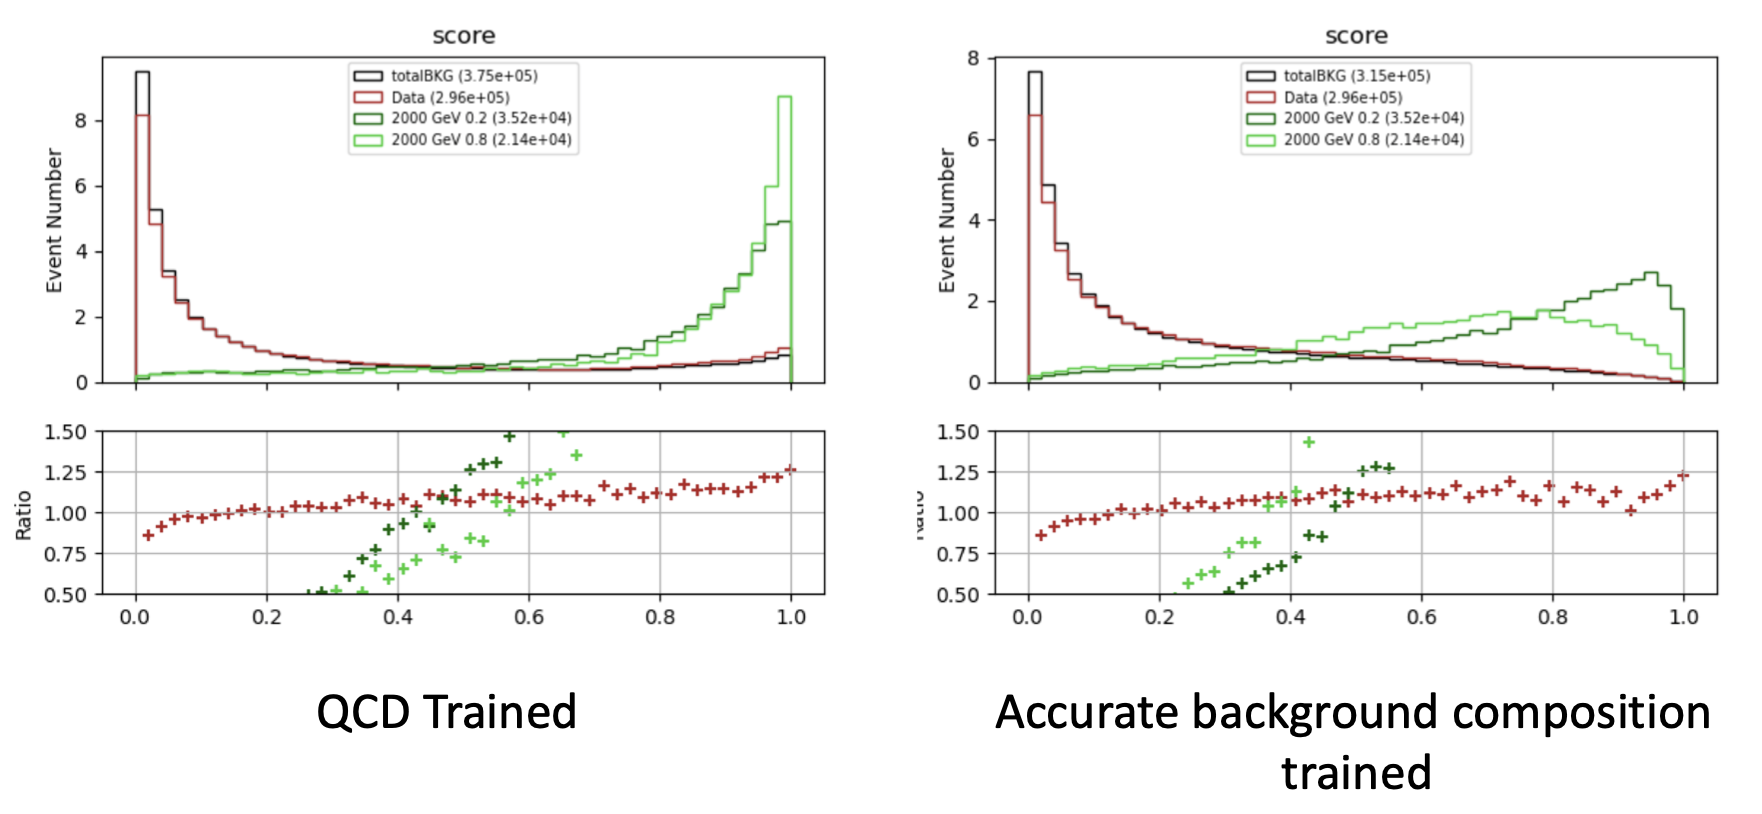
\includegraphics[width=0.98\textwidth]{figures/ml/pfn_MC_training_mixture}
    \caption{PFN score for full-background MC (black), data (red), and 2 representative signal points (green). The left plot is from a QCD-only training, while the right plot is from a full-background training. The histograms have been normalized to visualize the shapes better - the actual number of plotted events is shown in the legend. In the left plot we observe that both signal points are strongly classified as signal-like. In the right plot we observe less background contamination in the high score region, but worse signal classification. Both PFN trainings were tested for their effect on the analysis sensitivity and the QCD-only training was found to be favorable. 
    \label{fig:pfn_MC_training_mixture}}
\end{figure}

500k QCD MC background events and 500k SVJ signal events are used to train the network. The network is trained for 100 epochs. 20\% of the training events are used for training validation. Figure~\ref{fig:pfn_loss} shows the loss during training, which is stable and shows no indication of overtraining, and the final score that provides signal-background discrimination.

\begin{figure}[!htbp]
\centering
   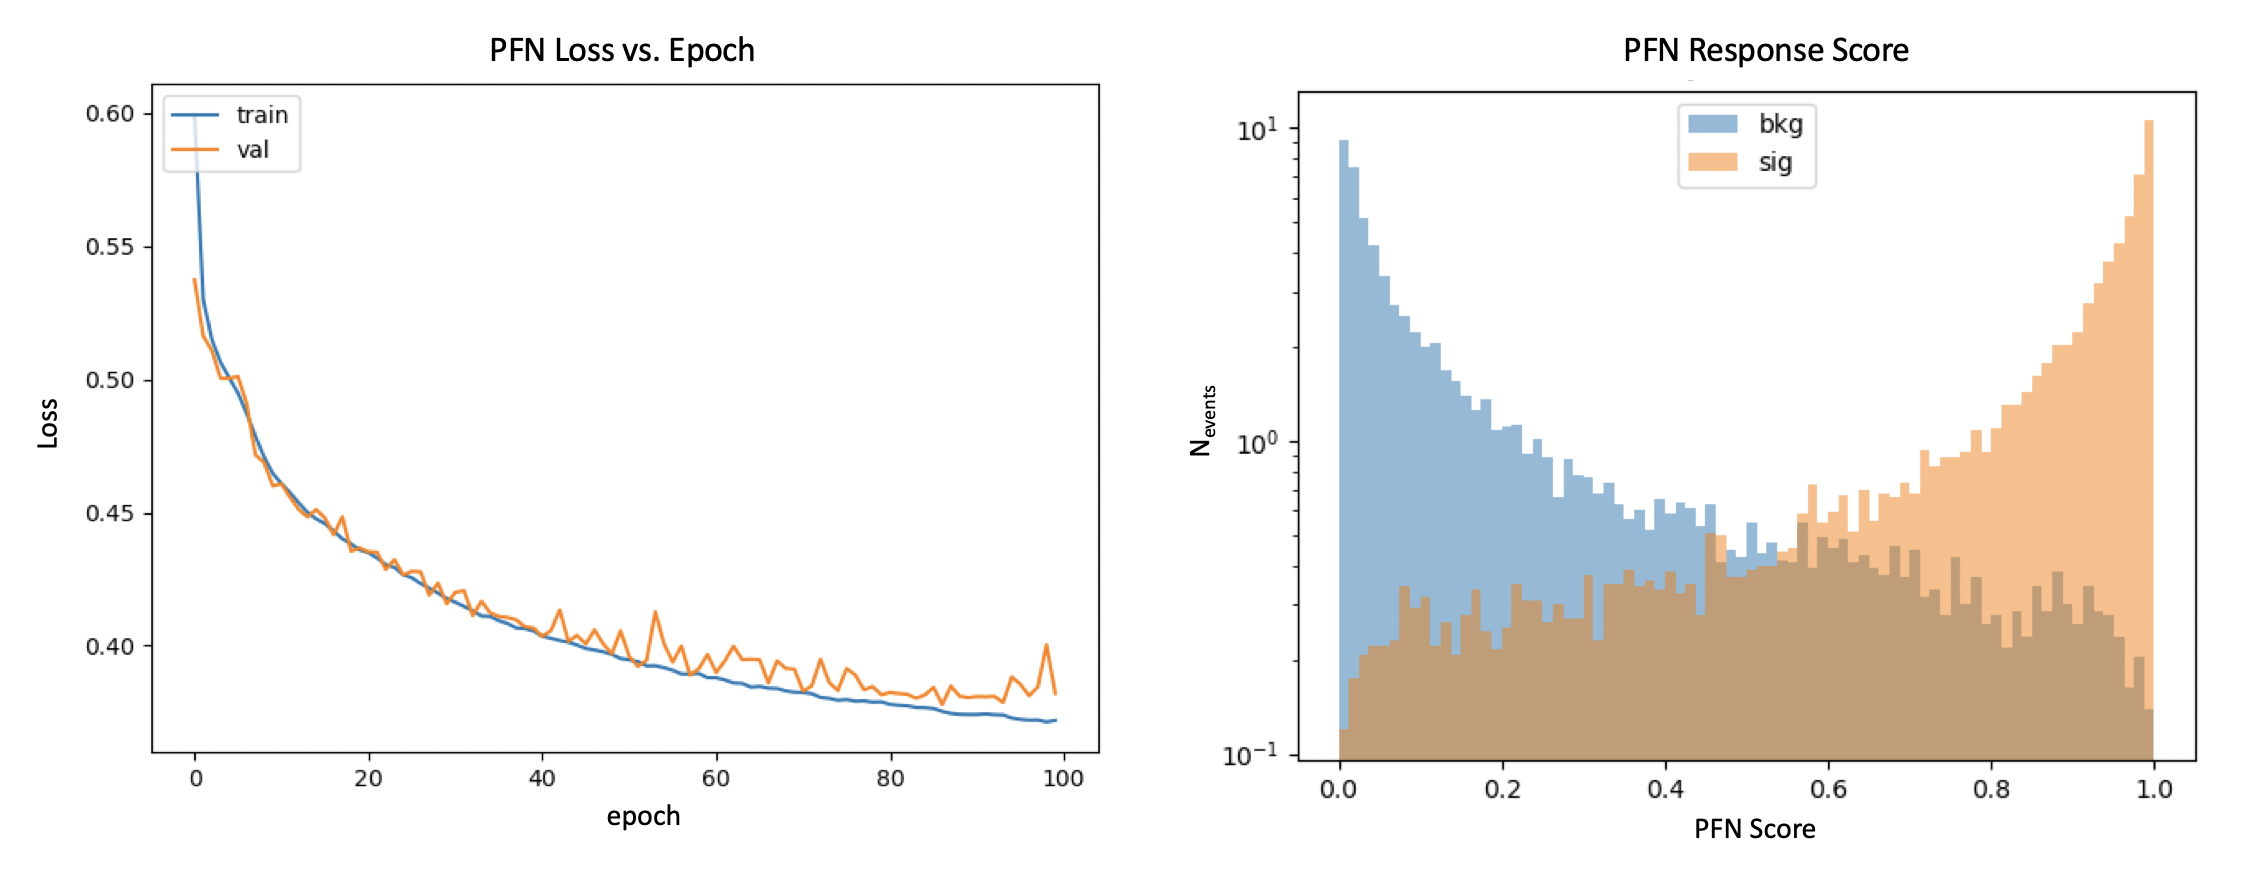
\includegraphics[width=0.9\textwidth]{figures/ml/pfn_loss_score}    
    \caption{PFN architecture loss during training as a function of epoch (left) and the evaluated score for signal and background training samples (right). The loss vs. epoch plot shows that the network is not overtrained. The score plot shows a good separation between signal and background.
    \label{fig:pfn_loss}}
\end{figure}

Optimization studies were performed on the PFN, varying the number of training epochs, number of training events, learning rate, number of nodes, and dimension of the $\Phi$ basis. A summary of these studies is presented in Appendix~\ref{app:pfn_qp}. The model presented here represents an optimal choice across these parameters.

%--------------------
\subsection{Performance}
\label{sec:pfn_performance}

The performance of the PFN is assessed via the AUC for each SVJ signal point.
Although the PFN is trained against QCD MC only, the performance is evaluated using data as the background sample, since the ultimate task of the PFN is to separate SVJ signals from data, which is dominated by SM processes.

Figure~\ref{fig:pfn_roc} shows the ROC curve of one such signal point, illustrating a smooth response.
Figure~\ref{fig:pfn_AUC_score_grid} shows the AUC of the PFN across the SVJ signal grid, demonstrating that AUC $>0.5$ is satisfied for all SVJ signals.

\begin{figure}[!htbp]
\centering
   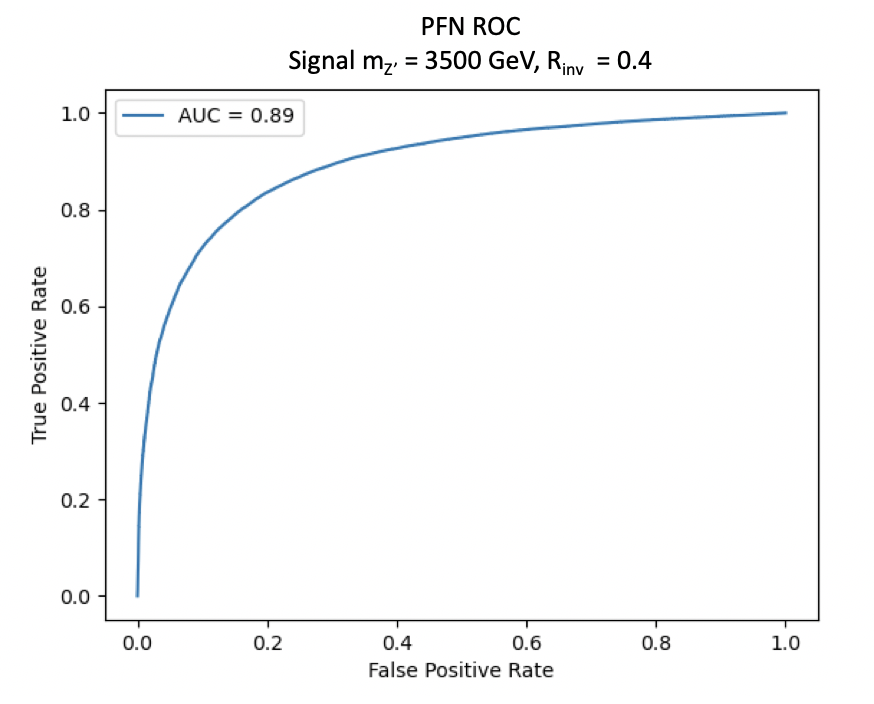
\includegraphics[width=0.7\textwidth]{figures/ml/pfn_roc}
    \caption{ROC for the PFN, using SVJ signal events (true positive) and data (false positive).
    \label{fig:pfn_roc}}
\end{figure}

\begin{figure}[!htbp]
\centering
   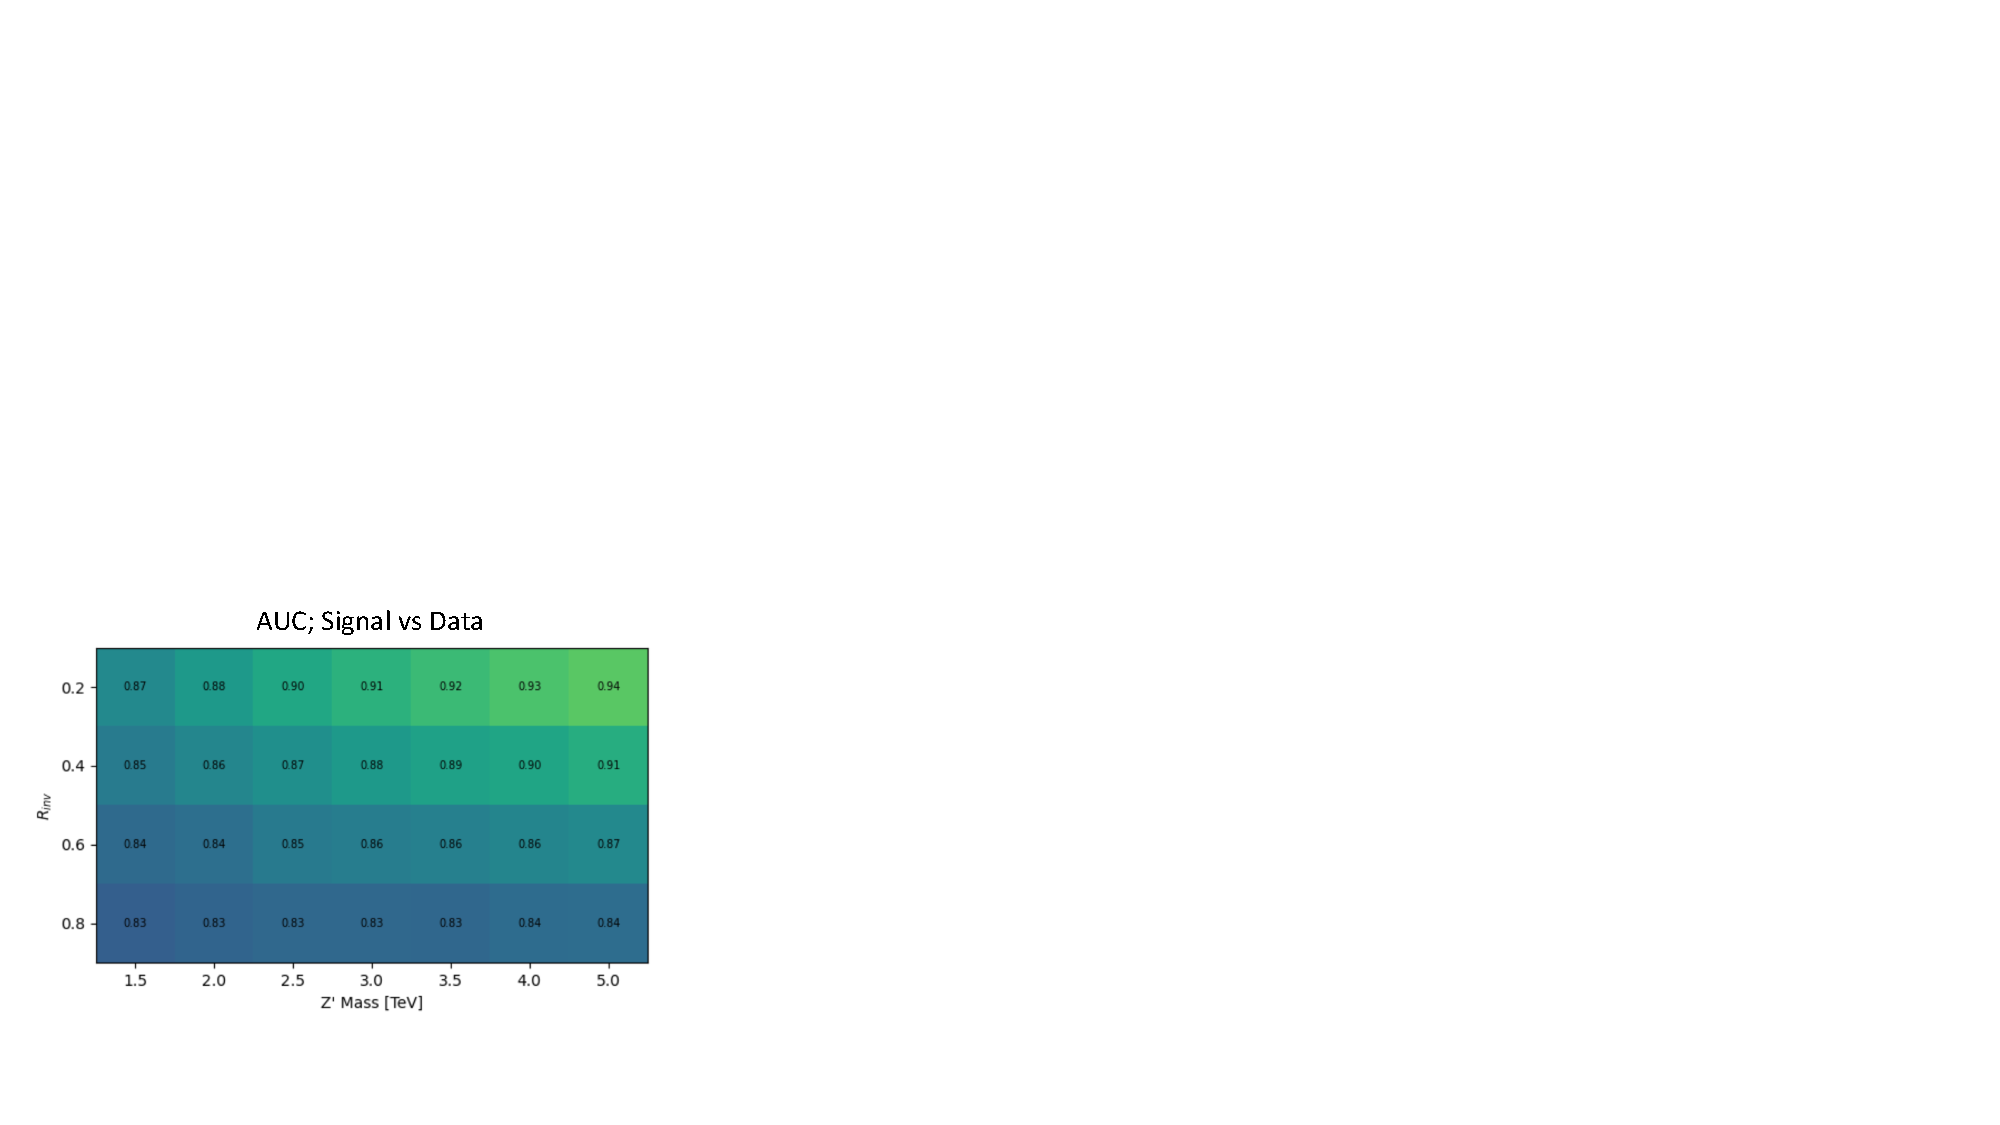
\includegraphics[width=0.7\textwidth]{figures/ml/pfn_AUC_grid}
    \caption{AUC for the PFN, shown for each signal in the SVJ grid.
    \label{fig:pfn_AUC_score_grid}}
\end{figure}

Figure~\ref{fig:pfn_score_all} shows the output score distribution for data and four signals, illustrating the range of scores received by data events in comparison to signal events.
As expected, most data events receive a background-like score (close to 0.0), indicating that the data is dominated by SM processes consistent with the background.
Most signal events receive a signal-like score (close to 1.0).
An optimization procedure determined that a selection of \textbf{PFN score > 0.6} can improve signal sensitivity across the grid.
The optimization procedure considered the cut that would maximize sensitivity as measured by $s/\sqrt{b}$, where $s$ the number of signal events accepted and $b$ is the number of background events selected.
This score selection is incorporated into the analysis design described in Chapter~\ref{ch:analysis}. 

\begin{figure}[!htbp]
\centering
   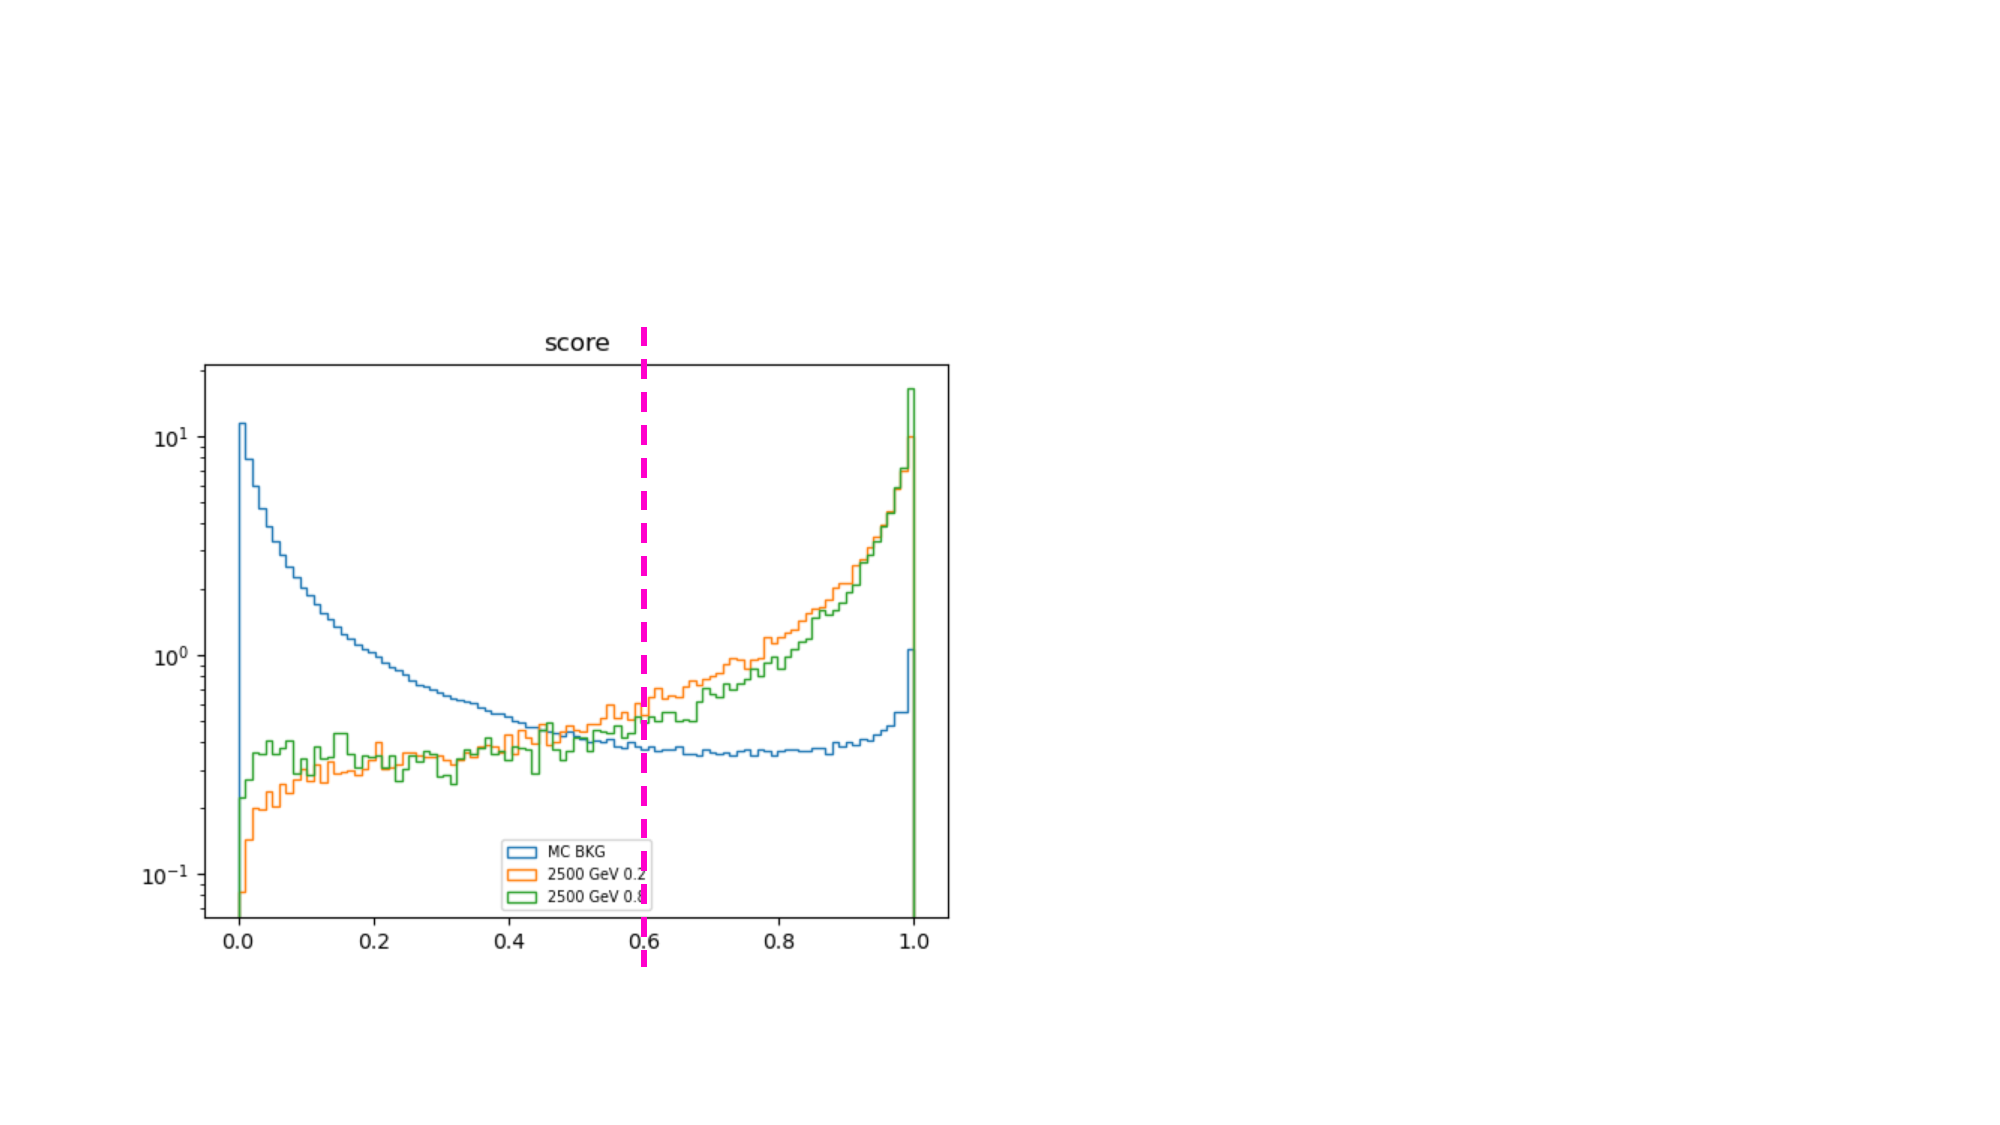
\includegraphics[width=0.5\textwidth]{figures/ml/pfn_score_all}
   \caption{Illustration of the PFN score selection, showing the separation between data (black) and 4 signal points (blue and green). The legend information takes the form ``$m_{Z'}$ \rinv'' for the signal. The PFN score selection value is shown by the pink line. Only events with a score > 0.6 will be accepted for use in the analysis. We see that most background (data) is rejected, while most signal is accepted.}
   \label{fig:pfn_score_all}
\end{figure}

%The agreement between data and background MC is illustrated in Figure~\ref{fig:mlscore_effComp}. The agreement is generally good, although some slope is observed in the ratio between the two shapes. The data has a small bias towards higher PFN scores compared to the background MC. However, the PFN score is only used in the analysis to make a selection on data events (PFN score > 0.6). The difference in selection efficiency for data and background MC <5.0\%, which is negligible for this analysis. 
%\begin{figure}[!htbp]
%\centering
%   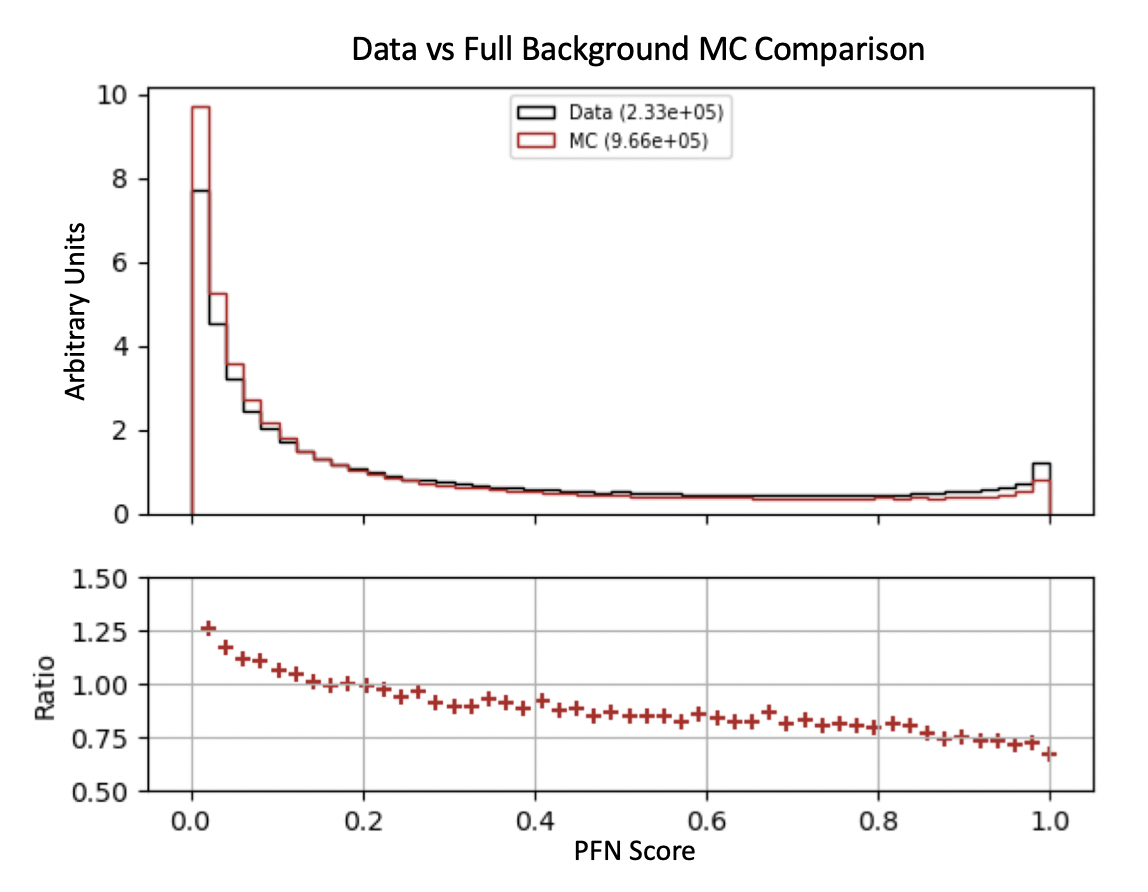
\includegraphics[width=0.5\textwidth]{figures/ml/mlscore_effComp}
%    \caption{PFN score comparison between normalized data and background MC shapes. Some slope is observed in the ratio panel.
%    \label{fig:mlscore_effComp}}
%\end{figure}

\clearpage


\section{ANTELOPE (Semi-supervised)}
\label{subsec:unsupervised}

The semi-supervised machine learning approach broadens the discovery potential of the search through the use of data-driven training, where no signal model is provided.
While broad sensitivity is a general goal of LHC searches, it is particularly motivated in the case of dark QCD models, which can lead to widely varying topologies depending on the values of model parameters.

%--------------------
\subsection{Architecture Fundamentals}
The model-independent search region of this analysis is implemented with a novel ML approach that builds on the PFN architecture to construct a tool that is capable of performing low-level anomaly detection with permutation-invariant inputs.
This tool, referred to as \textbf{ANomaly deTEction on particLe flOw latent sPacE (ANTELOPE)}, is a custom solution designed for this analysis.

Figure~\ref{fig:antelope_arch} provides a diagram of the ANTELOPE architecture. ANTELOPE uses the trained PFN network described in the previous section to generate a permutation invariant event representation $\mathcal{O}$ from track level inputs. The $\mathcal{O}$ basis is used as the input for a \textit{variational autoencoder} (VAE). A VAE is a common variation of a standard AE; the AE becomes \textit{variational} if the latent space is constructed through Gaussian sampling rather than a vector of weights, as described further in Ref.~\cite{vae2}. VAEs have been used in previous ATLAS searches to model low-level particle information, such as the search presented in Ref.~\cite{yxh} which used the recurrent architecture described in Ref.~\cite{vrnn}. One of the limitations of a recurrent architecture is the need to order the low-level inputs, which affects the performance of the tool. Jet track information is intrinsically unordered, and therefore a permutation invariant approach removes this element of arbitrary decision making from the modeling process. 

\begin{figure}[!htbp]
\centering
   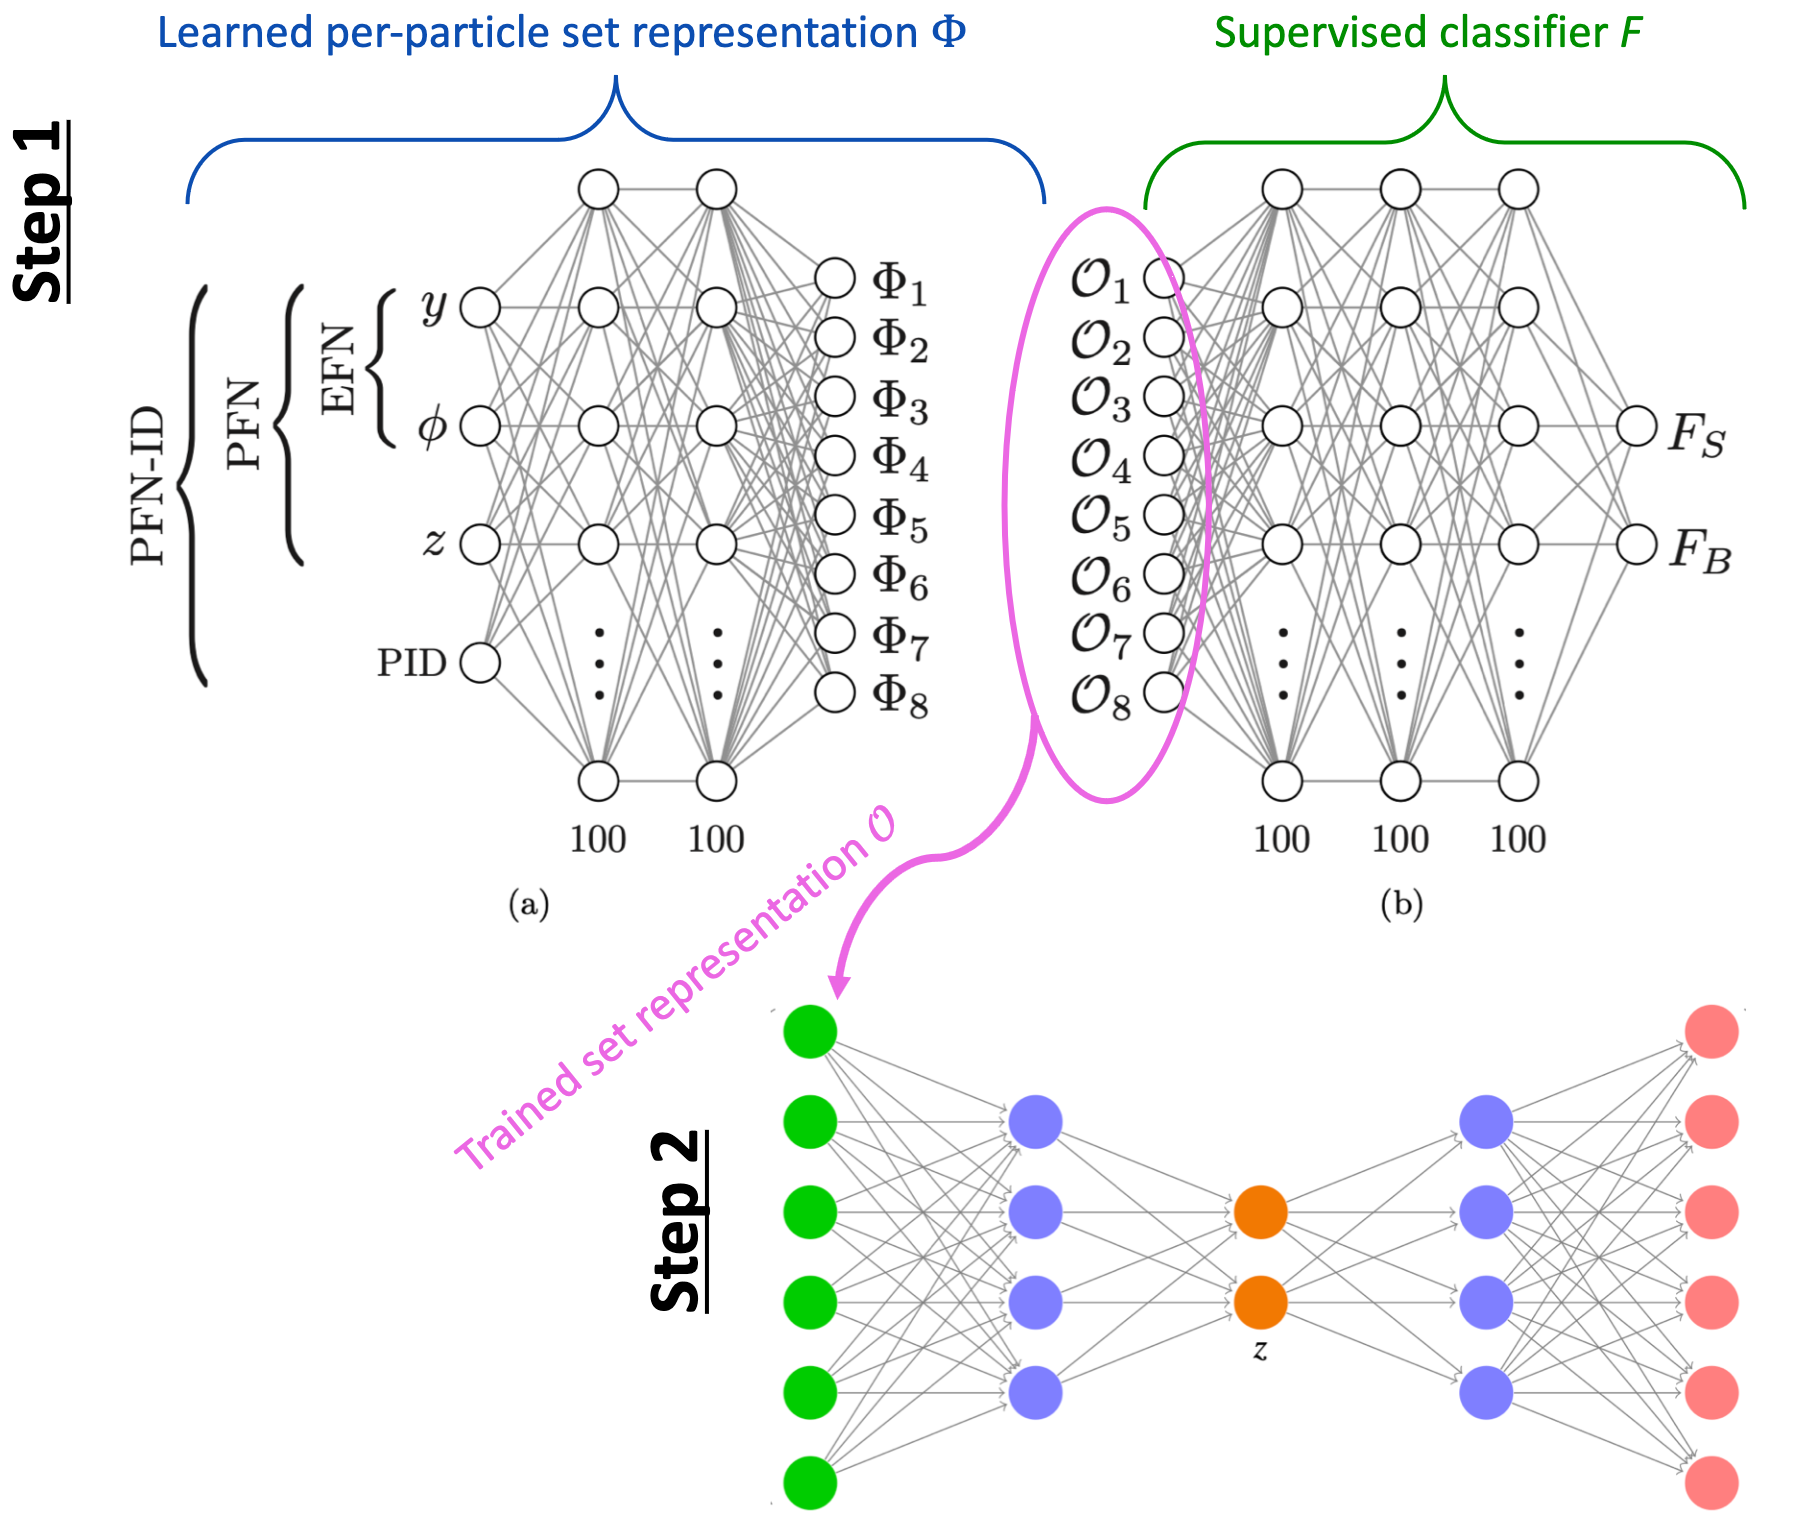
\includegraphics[width=0.9\textwidth]{figures/ml/antelope_arch}
    \caption{An annotated diagram of the ANTELOPE architecture. Step 1 illustrates the PFN which is fully trained before its use in the ANTELOPE network. Step 2 illustrates the variational auto-encoder. The Gaussian sampling of the latent space is shown, illustrating how the VAE differs from the AE shown in Figure~\ref{fig:ae}. 
    \label{fig:antelope_arch}}
\end{figure}

The input to ANTELOPE architecture is the same 6 track variables for the leading two jets, as presented in Section~\ref{sec:input_model}. The track information is encoded to the PFN $\mathcal{O}$ event representation using the pre-trained $\Phi$ neural network (trained according to the steps outline in Section~\ref{sec:pfn_training}). The VAE is then trained in an \textit{unsupervised} way using inputs encoded to $\mathcal{O}$ from data events only. Here \textit{unsupervised} means that the VAE is given no knowledge of the signal model during training. There is implicit knowledge of the signal model in the $\mathcal{O}$ encoding, so the full ANTELOPE network is considered semi-supervised, while the VAE component is unsupervised. A visual example of the $\mathcal{O}$ input to the VAE portion of the ANTELOPE is given in Figure~\ref{fig:antelope_input_rep}. 

\begin{figure}[!htbp]
\centering
   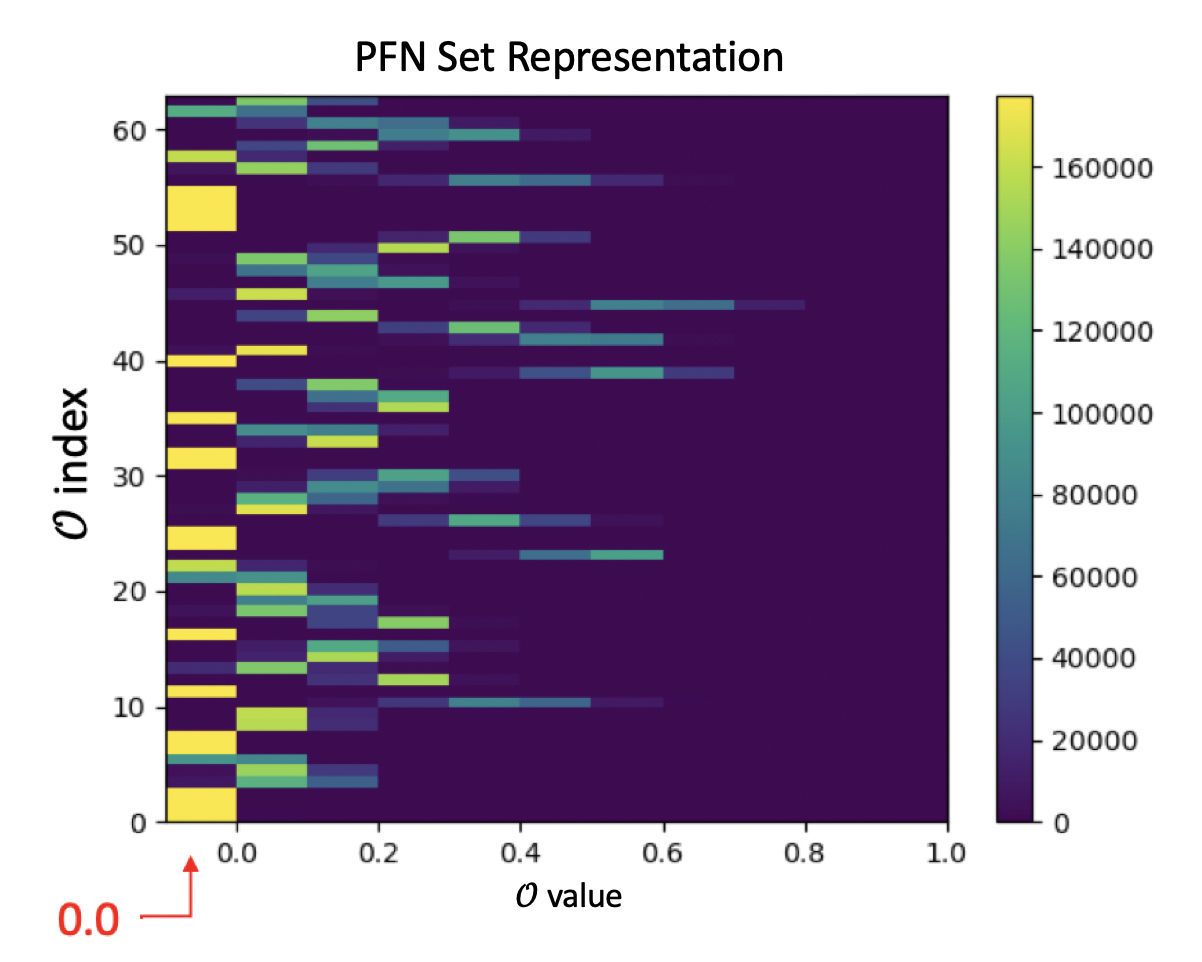
\includegraphics[width=0.7\textwidth]{figures/ml/antelope_input_rep}
    \caption{A visual representation of the 64 PFN $\mathcal{O}$ which create the input for the VAE component of ANTELOPE. The plot is 2D histogram of the PFN $\mathcal{O}$ index (0-63) versus the value assumed by that index. Many entries have a $\mathcal{O}$ value of exactly 0.0. To visually separate these from entries with a small but non-zero $\mathcal{O}$ value, any entries with value = 0.0 are moved to value = -0.01 (leftmost column) for the purpose of the plot only.
    \label{fig:antelope_input_rep}}
\end{figure}

The VAE is trained to minimize the reconstruction error, or the difference between its input and output layer. This pushes it to uncover patterns in the data, which is predominantly composed of SM processes. Any rare events in the data which present patterns inconsistent with the majority of the data will receive a higher reconstruction error. This error is used to create the anomaly score. 

%--------------------
\subsection{Training}

The VAE stage of the ANTELOPE network is trained over 500k data events.
The input dimensionality of the VAE has to match the encoded $\Phi$ dimension of the PFN, in this case 64. 
The encoding portion of the VAE has a hidden layer with 32 nodes,  and a latent space dimension of 12.
The decoding portion has another hidden layer of 32 nodes, and the output layer has a dimension of 64 to match the input layer.
All layers use a \textsc{relu} activation~\cite{scikit-learn} except for the output layer which uses a \textsc{sigmoid} activation~\cite{scikit-learn}, to restrict the output between 0 and 1.
As in the PFN, the Adam optimizer~\cite{adam}~\cite{scikit-learn} is used.

The network is trained for 50 epochs, with a learning rate of 0.00001. 
The VAE was observed to need a very small learning rate to effectively minimize the loss.
The loss $\mathcal{L}$ is the sum of two terms, the mean-squared error (MSE) of input-output reconstruction, and the Kullback-Leibler divergence (KLD).

\begin{equation}
\label{eq:vrnnloss}
\mathcal{L} = \sum_i L_i = \sum_i | \Phi_i^2 - \Phi\prime_i |^2 + \lambda D_{\text{KL}}
\end{equation}

Figure~\ref{fig:antelope_loss} shows the loss during training.
The validation events are seen to have a lower loss than the training events, indicating there is no issue with overtraining.
\begin{figure}[!htbp]
\centering
   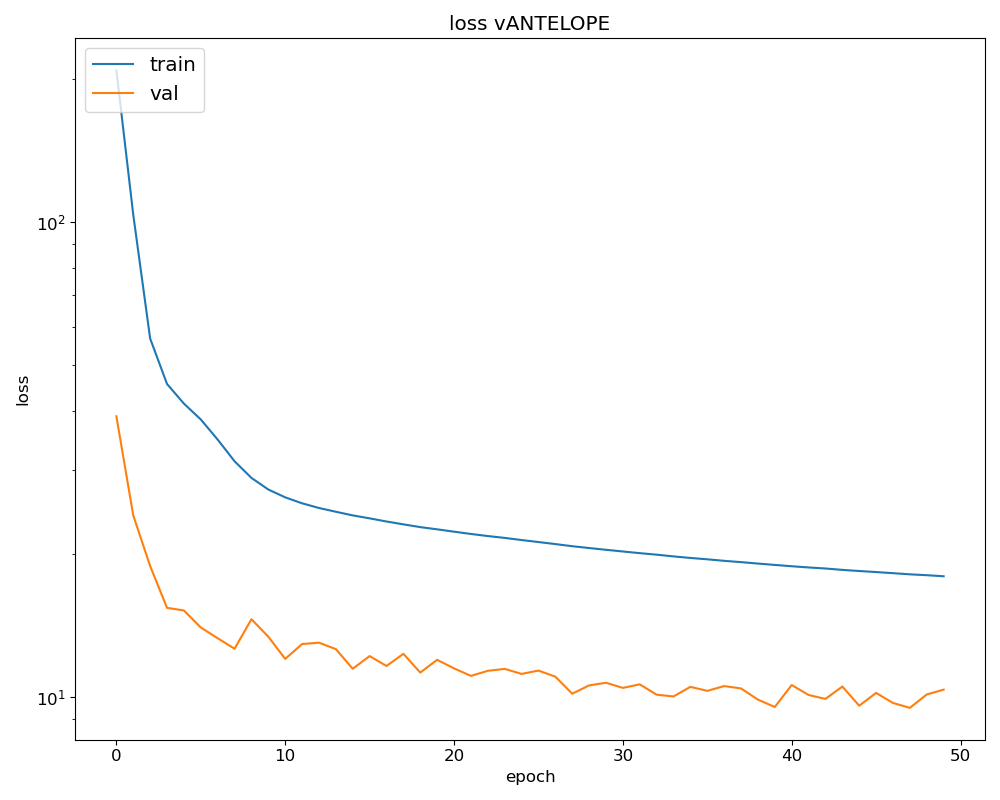
\includegraphics[width=0.5\textwidth]{figures/ml/antelope_loss}    
    \caption{ANTELOPE architecture loss during training as a function of epoch.
    \label{fig:antelope_loss}}
\end{figure}


%--------------------
\subsection{Performance}
\label{subsec:antelope_perf}

As with the PFN, the ANTELOPE performance is assessed via the ROC and AUC. 
Figure~\ref{fig:antelope_score} shows the anomaly score and an example ROC curve.
The anomaly score is calculated from the loss as defined in \ref{eq:vrnnloss}.
The score is produced by applying a sigmoid function to the loss to restrict its output between 0.0 and 1.0:

\begin{equation}
\label{eq:asfunc}
a = \frac{1}{1+e^{-\mathcal{L}}}
\end{equation}
where $a$ is the anomaly score and $\mathcal{L}$ is the VAE loss. Because the loss is always positive, the sigmoid transformation effectively restricts the anomaly score range between 0.5 and 1.0. The anomaly score is observed to range between 0.6 and 1.0, as the reconstruction loss is always non-zero. Following a similar sensitivity optimization as presented for the PFN score selection in Section~\ref{sec:pfn_performance}, a selection of \textbf{anomaly score > 0.7} is chosen for use in the analysis.

\begin{figure}[!htbp]
\centering
   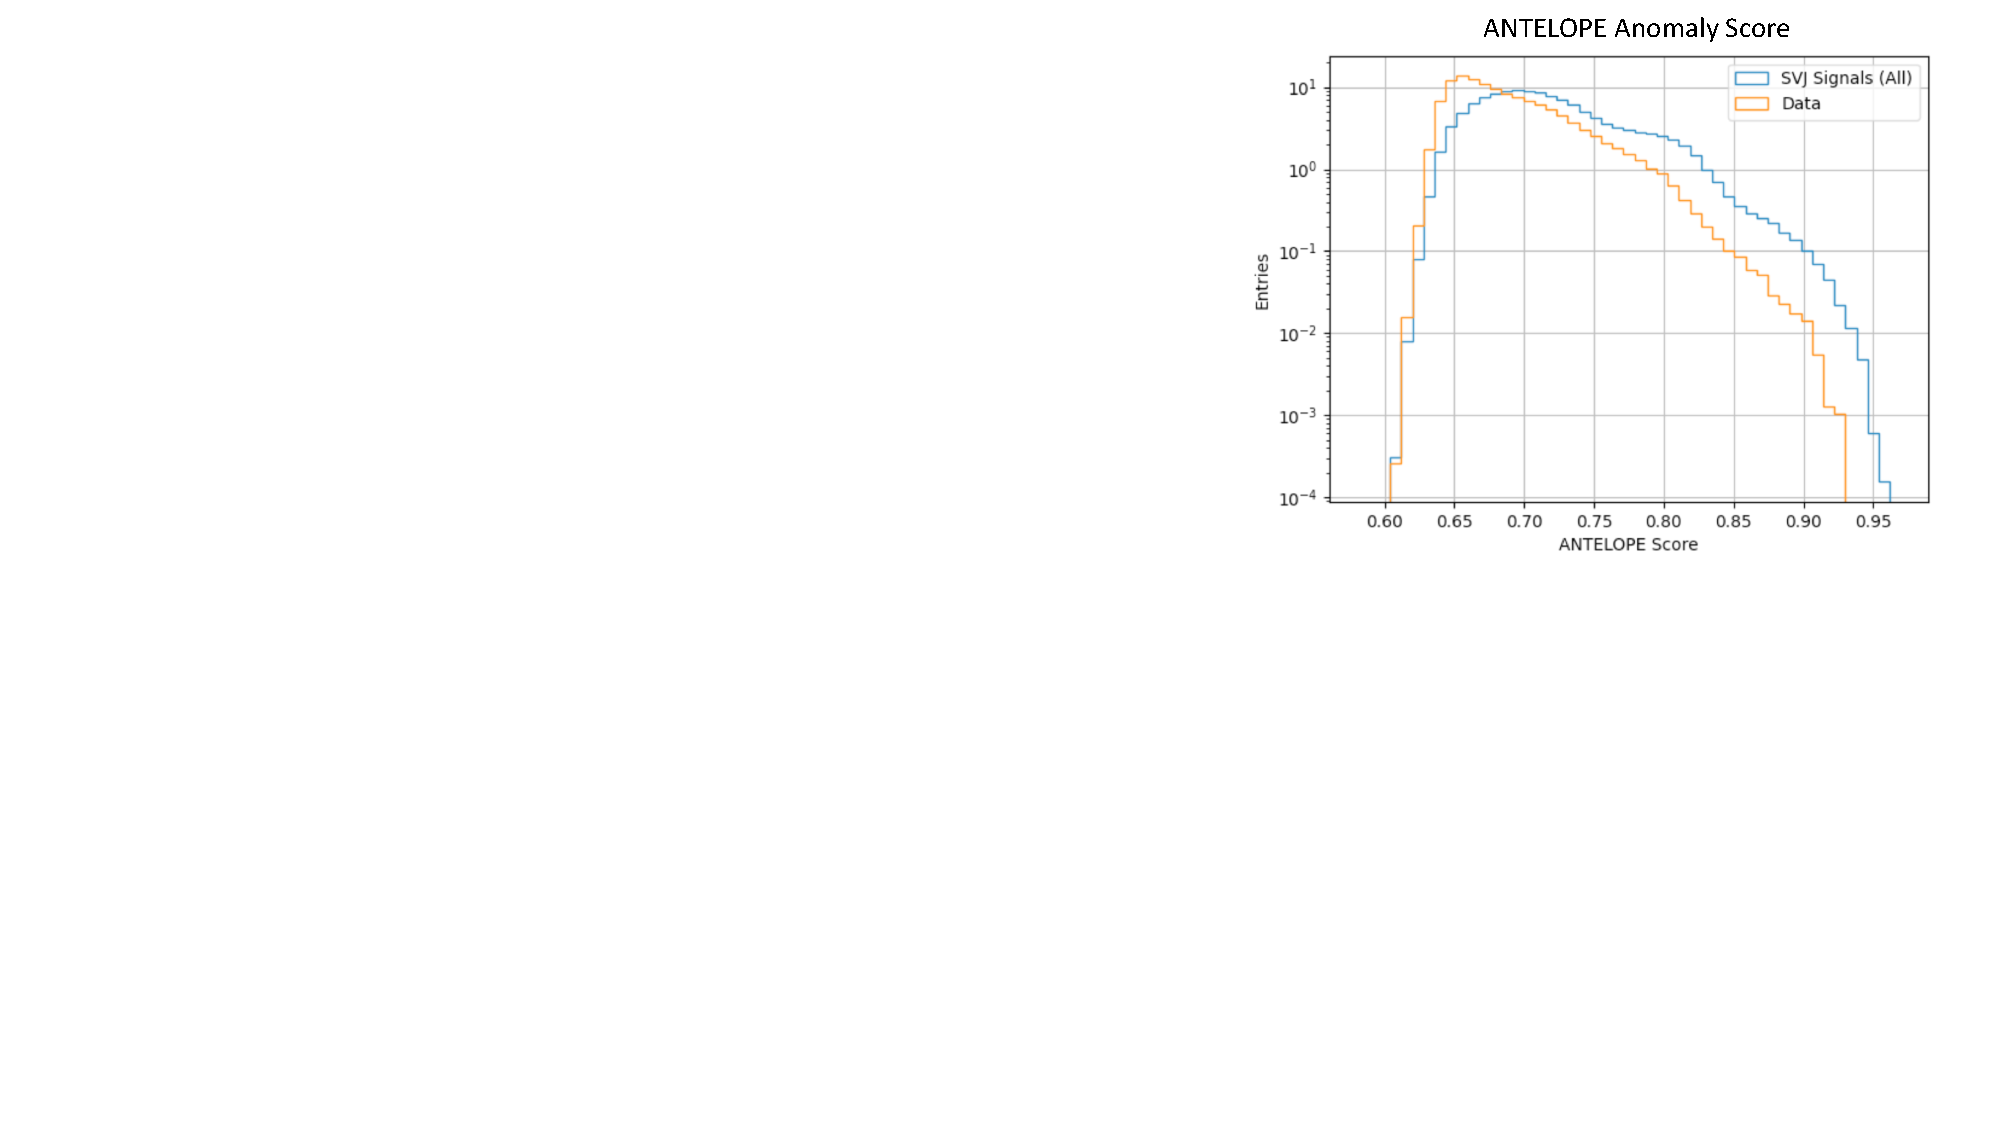
\includegraphics[width=0.48\textwidth]{figures/ml/antelope_score.pdf}
   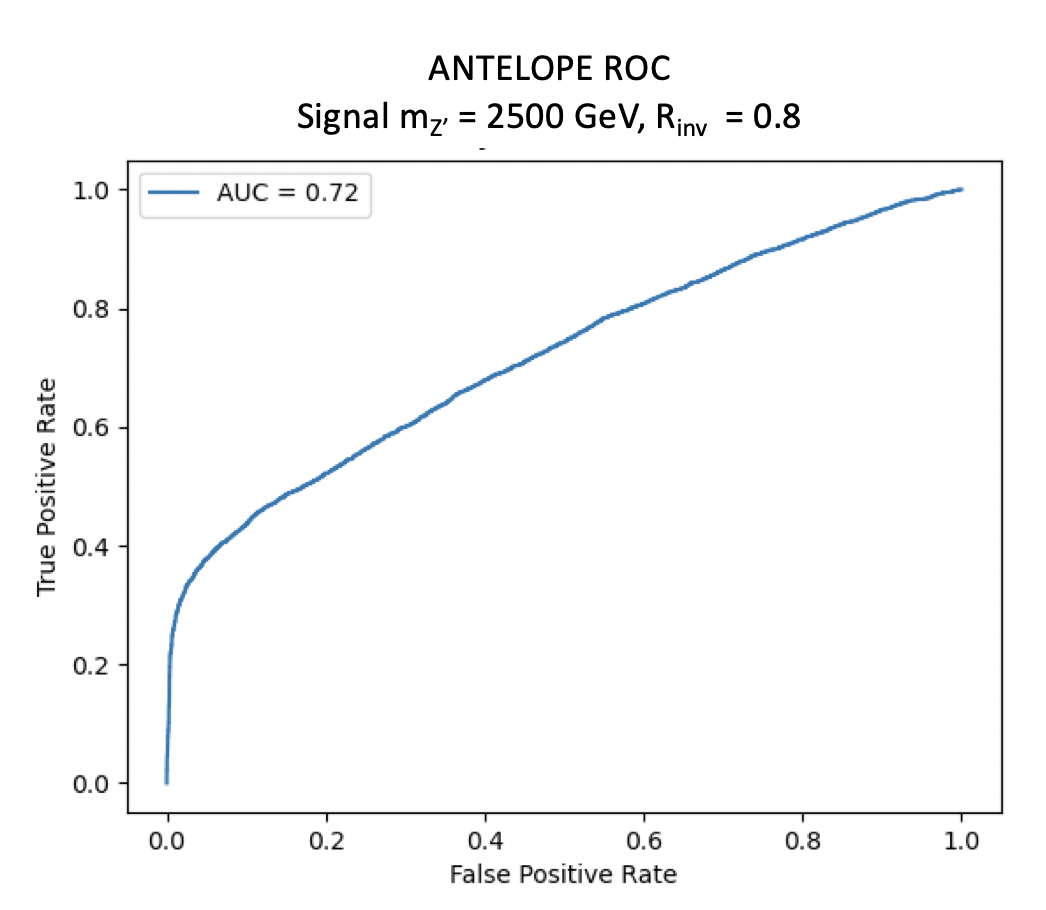
\includegraphics[width=0.48\textwidth]{figures/ml/antelope_roc}
    \caption{Anomaly score distribution (left), comparing all data (orange) and all SVJ signals (blue). The signals have a small but consistently higher score than the data, indicating that they are tagged as more anomalous by ANTELOPE. A ROC curve for an example signal point is also shown (right).
    \label{fig:antelope_score}}
\end{figure}

Figure~\ref{fig:antelope_AUC_score_grid} shows the AUC of the ANTELOPE across the SVJ signal grid, demonstrating discrimination capability across varying SVJ signal models.
Compared to the supervised PFN method, the ANTELOPE is not as performant (as expected due to the absence of signal model in training).
However, the network is seen provide separation between signal and background for all signal points, as evidenced by AUC $> 0.5$ across the signal grid.

\begin{figure}[!htbp]
\centering
   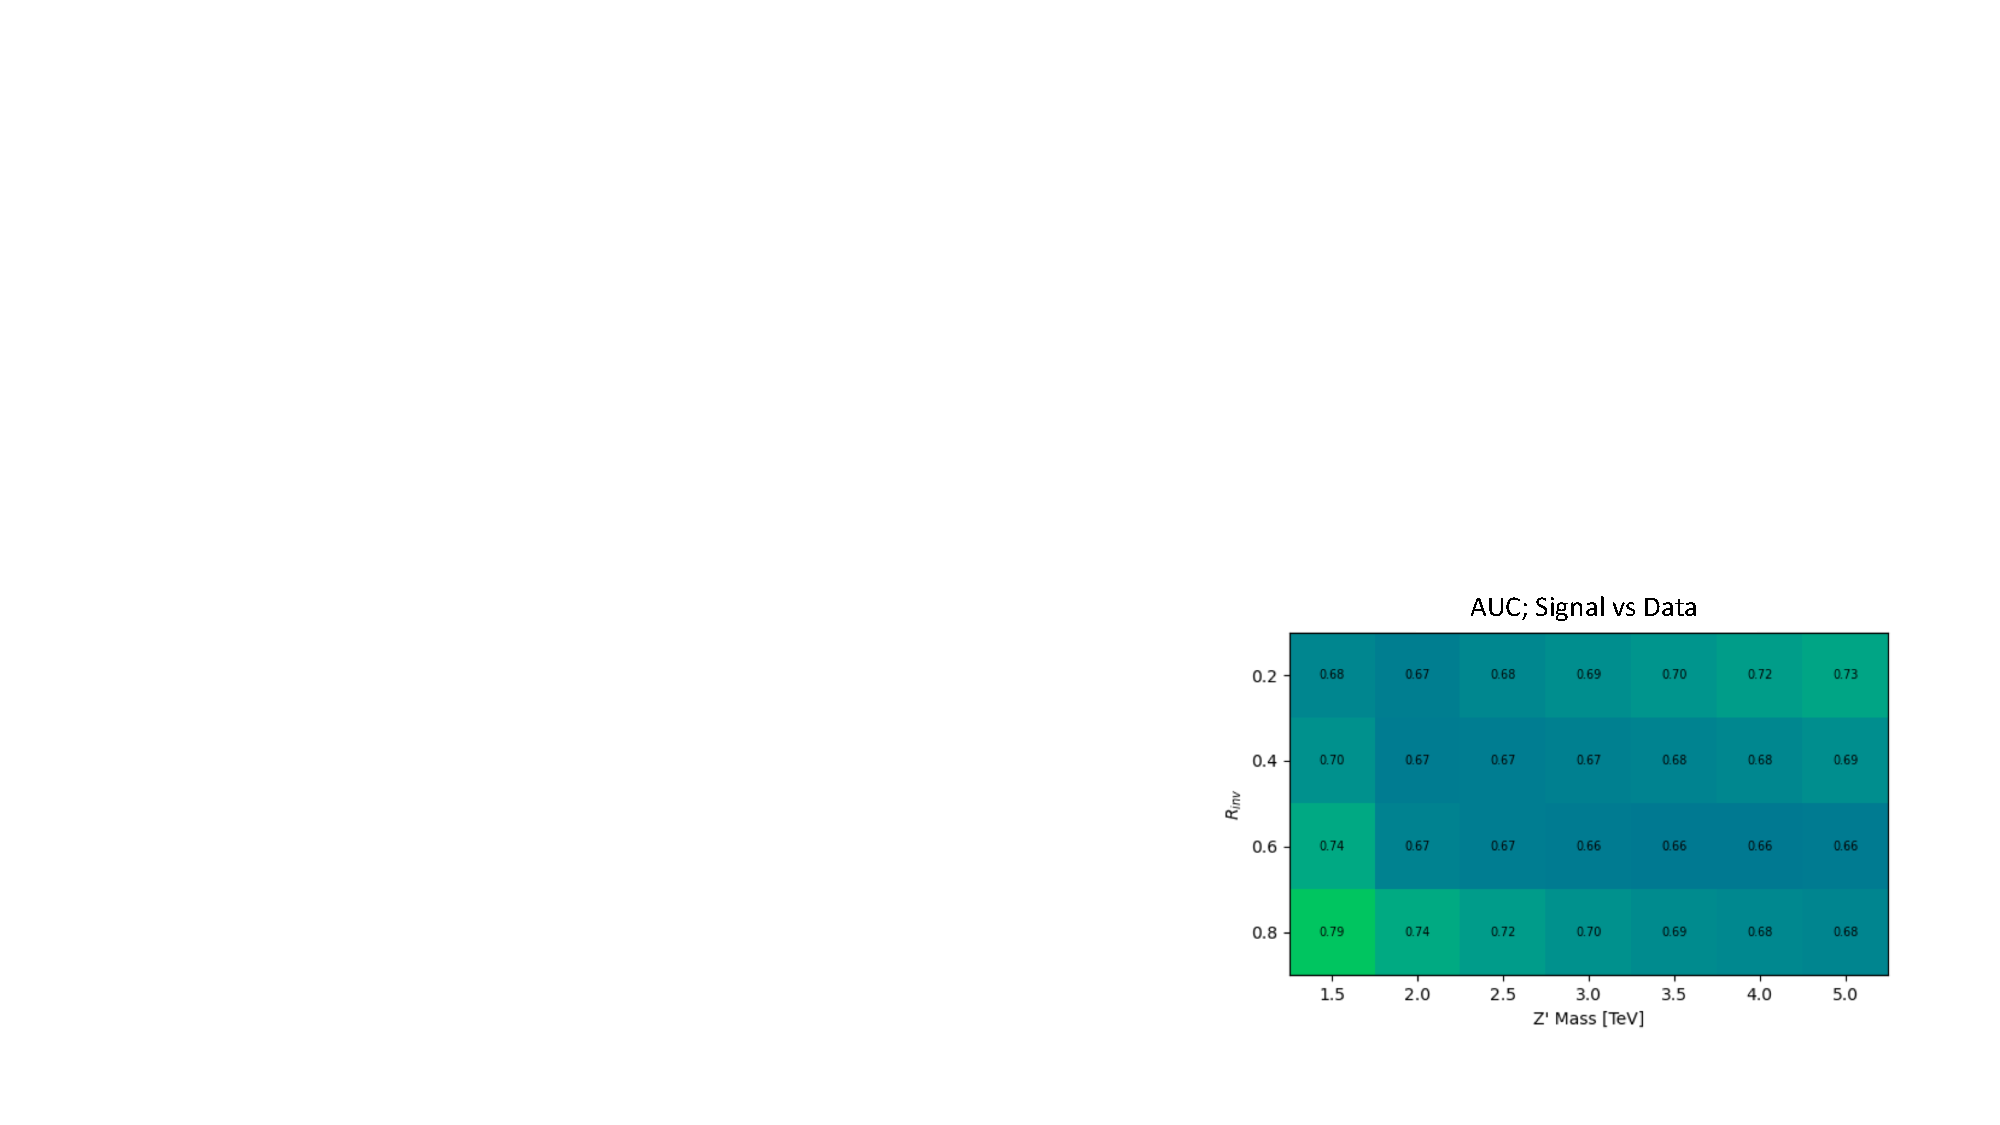
\includegraphics[width=0.7\textwidth]{figures/ml/antelope_AUC_score_grid}
    \caption{AUC from the ANTELOPE score for each signal in the SVJ grid.
    \label{fig:antelope_AUC_score_grid}}
\end{figure}

\paragraph{Model Independence} 

The unsupervised component of training the ANTELOPE network is expected to give it a more generalized sensitivity to new physics with \met~and jet activity, beyond the scope of the SVJ grid. 
To assess this, alternative signal models are evaluated with the trained ANTELOPE network.

The following alternate signal models were considered: 
\begin{itemize}
\item Z' $\rightarrow$ $t\bar{t}$ 
\item W' $\rightarrow$ WZ 
\item Gluino pair production $\rightarrow$ R-hadron + LSP (\met) with gluino masses 2000/3000 GeV, LSP mass 100 GeV, and lifetime 0.03 ns (LSP = \textit{lightest supersymmetric particle})
\item Emerging jets s-channel with mass 1000 GeV and lifetime 1ns 
\end{itemize}

Figure~\ref{fig:antelope_altsig} shows the distribution of these signals in the PFN score and the ANTELOPE anomaly score.
The benefit of the ANTELOPE in enhancing model independence is clearly seen through the boost in performance for certain non-SVJ signal models.
The gluino and emerging jet signals in particular are marked as highly anomalous by the ANTELOPE, but are marked as evenly background-like and signal-like by the PFN.
This observation demonstrates that the use of the ANTELOPE network in this analysis has the potential to expand our sensitivity to include alternate signal models that could be marked as highly anomalous with the anomaly score.

\begin{figure}[!htbp]
\centering
   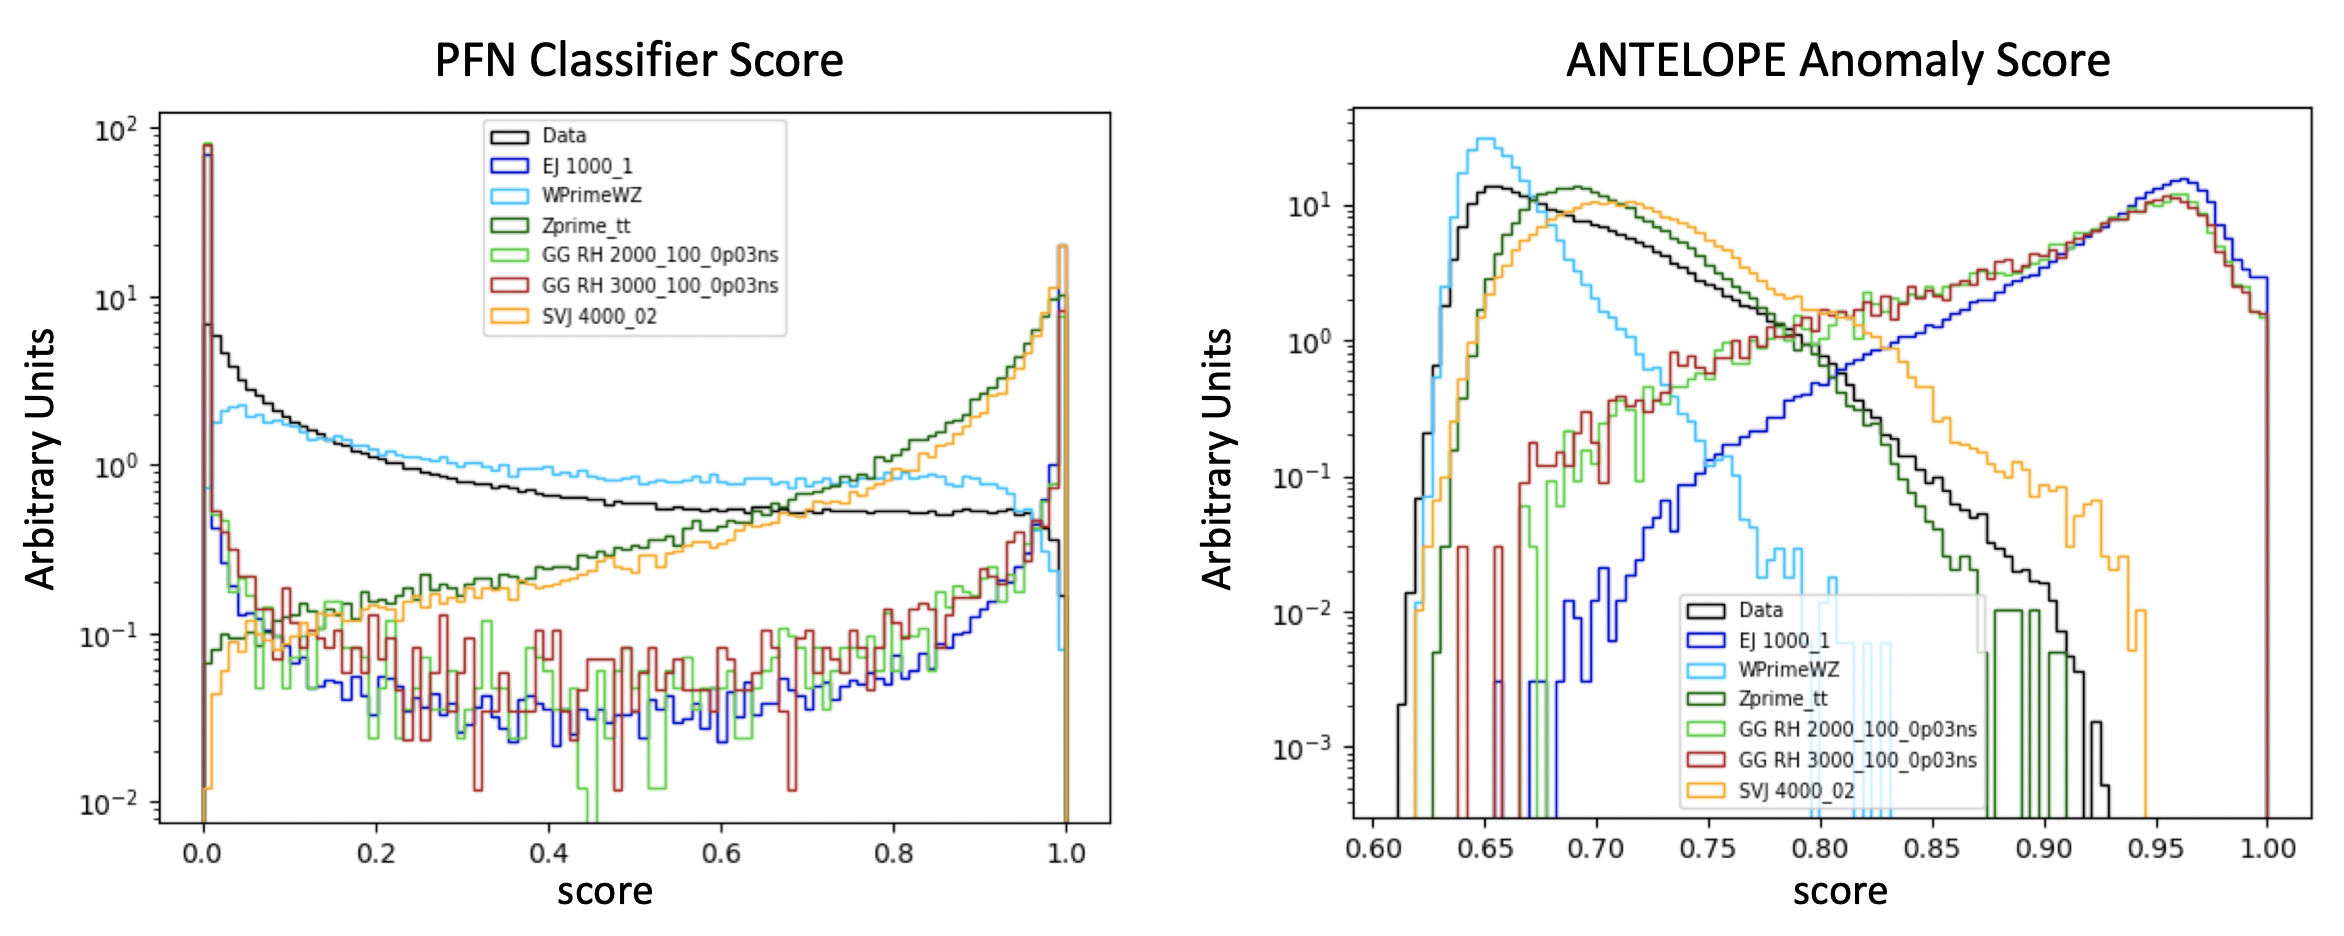
\includegraphics[width=0.98\textwidth]{figures/ml/antelope_vs_pfn_score}
    \caption{Comparing data and the alternate signal models for the PFN score (left) and ANTELOPE score (right). The emerging jet signal (dark blue) and gluino R-hadron signals (red, light green) are an example of the advantage of the model-independent ANTELOPE approach. These signals have a bimodal shape in PFN score but are clearly tagged with a high anomaly score by the ANTELOPE.
    \label{fig:antelope_altsig}}
\end{figure}





